%% 
%% Copyright 2007-2020 Elsevier Ltd
%% 
%% This file is part of the 'Elsarticle Bundle'.
%% ---------------------------------------------
%% 
%% It may be distributed under the conditions of the LaTeX Project Public
%% License, either version 1.2 of this license or (at your option) any
%% later version.  The latest version of this license is in
%%    http://www.latex-project.org/lppl.txt
%% and version 1.2 or later is part of all distributions of LaTeX
%% version 1999/12/01 or later.
%% 
%% The list of all files belonging to the 'Elsarticle Bundle' is
%% given in the file `manifest.txt'.
%% 

%% Template article for Elsevier's document class `elsarticle'
%% with numbered style bibliographic references
%% SP 2008/03/01
%%
%% 
%%
%% $Id: elsarticle-template-num.tex 190 2020-11-23 11:12:32Z rishi $
%%
%%
\documentclass[preprint,12pt]{elsarticle}

%% Use the option review to obtain double line spacing
%% \documentclass[authoryear,preprint,review,12pt]{elsarticle}

%% Use the options 1p,twocolumn; 3p; 3p,twocolumn; 5p; or 5p,twocolumn
%% for a journal layout:
%% \documentclass[final,1p,times]{elsarticle}
%% \documentclass[final,1p,times,twocolumn]{elsarticle}
%% \documentclass[final,3p,times]{elsarticle}
%% \documentclass[final,3p,times,twocolumn]{elsarticle}
%% \documentclass[final,5p,times]{elsarticle}
%% \documentclass[final,5p,times,twocolumn]{elsarticle}

%% For including figures, graphicx.sty has been loaded in
%% elsarticle.cls. If you prefer to use the old commands
%% please give \usepackage{epsfig}

%% The amssymb package provides various useful mathematical symbols
\usepackage{hyperref}
\usepackage{amssymb}
\usepackage{multirow}
\usepackage{booktabs}
\usepackage{comment}
\usepackage{xcolor}
\usepackage[T1]{fontenc}
\usepackage{graphicx}
\usepackage{booktabs}
\usepackage{amsmath}
\usepackage{amssymb}
\usepackage{comment}
\usepackage{hyperref}
\usepackage[section]{placeins}
\usepackage{tikz}
\usetikzlibrary{arrows.meta, positioning}
\hypersetup{
  colorlinks=true,
  linkcolor=blue,
  citecolor=blue,
  urlcolor=blue
}
%

%% The amsthm package provides extended theorem environments
%% \usepackage{amsthm}

%% The lineno packages adds line numbers. Start line numbering with
%% \begin{linenumbers}, end it with \end{linenumbers}. Or switch it on
%% for the whole article with \linenumbers.
%% \usepackage{lineno}

\journal{Artificial Intelligence in Medicine}

\begin{document}

\begin{frontmatter}

%% Title, authors and addresses

%% use the tnoteref command within \title for footnotes;
%% use the tnotetext command for theassociated footnote;
%% use the fnref command within \author or \address for footnotes;
%% use the fntext command for theassociated footnote;
%% use the corref command within \author for corresponding author footnotes;
%% use the cortext command for theassociated footnote;
%% use the ead command for the email address,
%% and the form \ead[url] for the home page:
%% \title{Title\tnoteref{label1}}
%% \tnotetext[label1]{}
%% \author{Name\corref{cor1}\fnref{label2}}
%% \ead{email address}
%% \ead[url]{home page}
%% \fntext[label2]{}
%% \cortext[cor1]{}
%% \affiliation{organization={},
%%             addressline={},
%%             city={},
%%             postcode={},
%%             state={},
%%             country={}}
%% \fntext[label3]{}

\title{AUC–Sensitivity Decoupling in Imbalanced ALS Prognosis:
An Explainable Machine Learning Study Using PRO-ACT}
\author[inst1,inst2,inst3]{Ivo Camacho }
\author[inst1]{Pedro Martins}
\author[inst1]{Maryam Abbasi \corref{cor1}}\ead{maryam@dei.uc.pt}
\cortext[cor1]{Corresponding author}



\affiliation[inst1]{organization={Centre for Informatics and Systems of the University of Coimbra},%Department and Organization
            addressline={Department of Informatics Engineering, University of Coimbra}, 
            city={Coimbra},
            country={Portugal}}
\affiliation[inst2]{organization={Polytechnic Institute of Coimbra, Applied Research Institute}, city={Coimbra}, country={Portugal}}
\affiliation[inst3]{organization={ Research Centre for Natural Resources Environment and Society, Polytechnic Institute of Coimbra}, city={Coimbra}, country={Portugal}}
%Research Centre for Natural Resources Environment and Society (CERNAS), Polytechnic Institute of Coimbra, Bencanta, 3045-601 Coimbra, Portugal



\begin{abstract}

Amyotrophic lateral sclerosis (ALS) is a progressive and fatal neurodegenerative
disease in which a subset of patients, termed Short Survivors, die within
24 months of symptom onset. Identifying this subgroup at diagnosis is
clinically relevant but is complicated by severe class imbalance: Short
Survivors typically represent fewer than 15\% of ALS cohorts, and standard
classifiers tend to overlook them in favour of the majority class.
This paper partially replicates and extends the ensemble-imbalance machine learning
framework of Papaiz et al.~\cite{Papaiz2024} using the publicly available
PRO-ACT clinical database. BalancedBagging significantly improves balanced
accuracy in six of seven classifiers (Bonferroni-corrected Wilcoxon test,
$p \leq 0.01$), with the MLP achieving the highest ensemble balanced accuracy
of 0.832. We then extend the framework by replacing grid search with Bayesian
hyperparameter optimisation (Optuna) and introducing LightGBM as a seventh
classifier across ten imbalance-handling strategies. On a held-out
partition drawn from the same PRO-ACT trial population, LightGBM with Random
Oversampling reaches an AUC of 0.923 and identifies 30 of 35 Short Survivors
(sensitivity 0.857). SVM with SMOTEENN achieves the highest sensitivity
(0.886) at a lower specificity (0.767). The MLP, despite leading
cross-validation AUC (0.915), identifies only one of those 35 patients at the
default decision threshold (sensitivity 0.029), illustrating that high AUC does
not guarantee adequate minority-class detection when a fixed threshold is applied.
Optimising the decision threshold using Youden's J statistic raises the MLP's
sensitivity to 0.486, yet it remains well below LightGBM+ROS, confirming the
AUC--sensitivity decoupling is structural rather than a calibration artefact.
SHAP analysis of both models identifies diagnostic delay and ALSFRS-R functional
decline slopes as the dominant predictors. All results are from an internal
held-out set; external validation on independent cohorts remains necessary.


\end{abstract}

%%Graphical abstract
\begin{graphicalabstract}
%\includegraphics{grabs}

\begin{center}
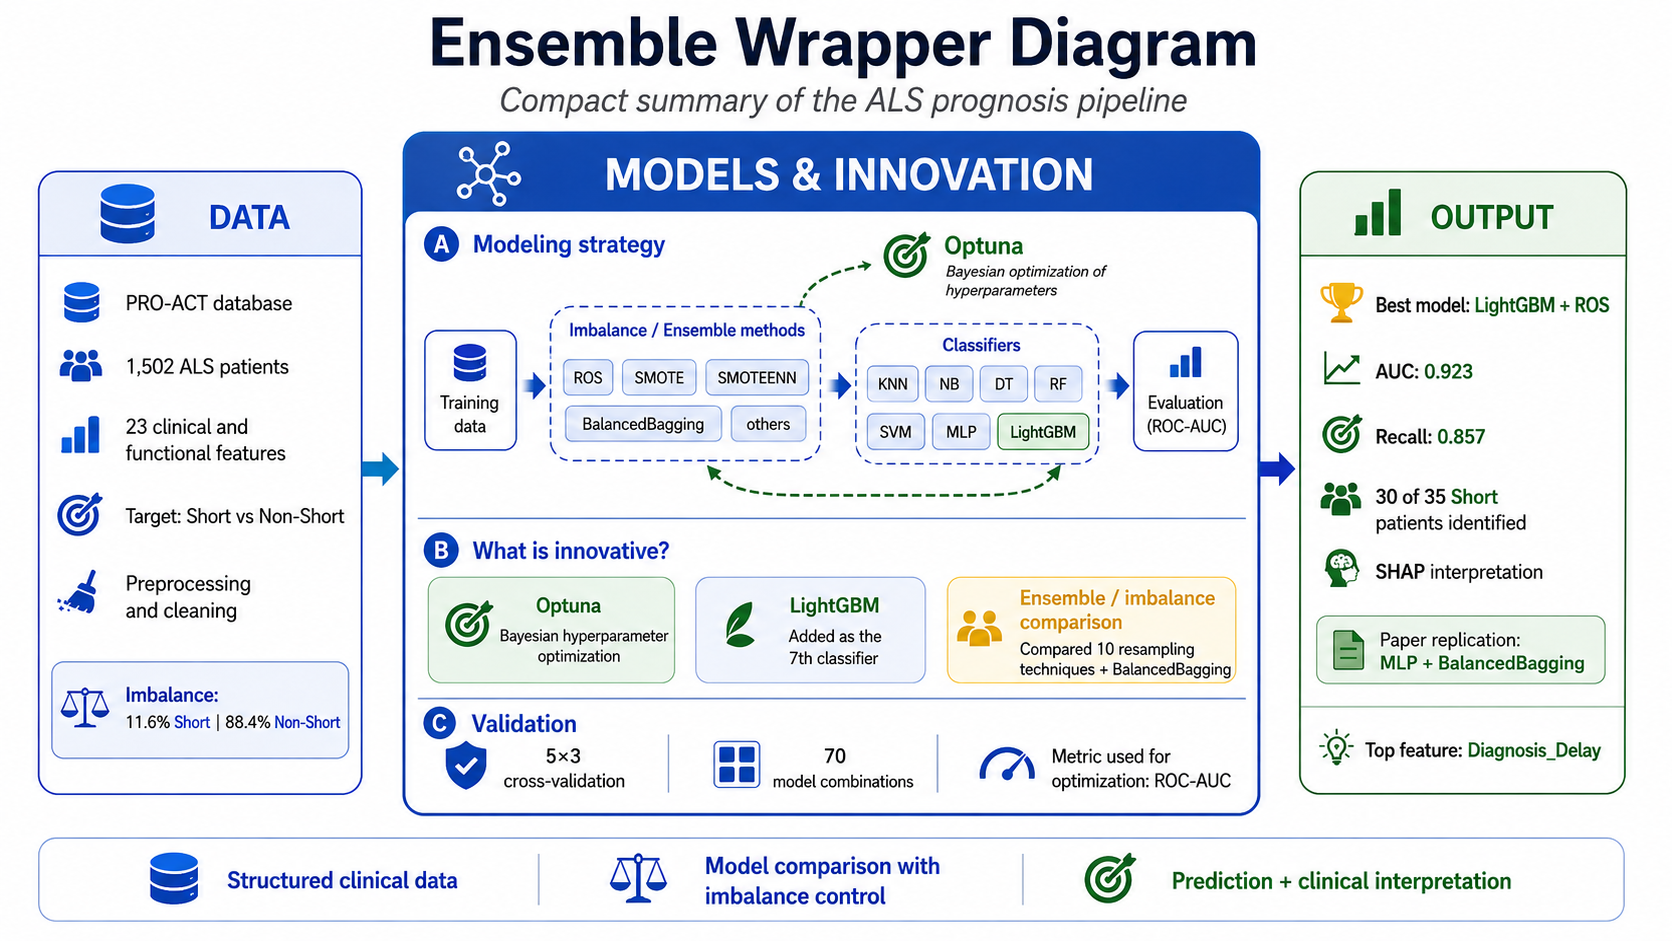
\includegraphics[width = 1 \textwidth]{figures/ensemble_wrapper.png}
\end{center}

\end{graphicalabstract}

%%Research highlights
\begin{highlights}
\item Ensemble imbalance-learning significantly improved ALS prognosis prediction across six of seven classifiers.
\item LightGBM with Random Oversampling achieved the best held-out performance (AUC = 0.923; sensitivity = 0.857).
\item High cross-validation AUC did not guarantee minority-class detection under severe class imbalance.
\item SHAP analysis identified diagnostic delay and ALSFRS-R decline slopes as dominant prognostic predictors.
\end{highlights}

\begin{keyword}
Amyotrophic Lateral Sclerosis \sep Machine Learning \sep Class
Imbalance \sep Ensemble Learning \sep LightGBM \sep Bayesian Optimisation
\sep SHAP \sep Explainability
\end{keyword}

\end{frontmatter}

%%\linenumbers

% ==========================================================================
\section{Introduction}
\label{sec:intro}
% ==========================================================================

Amyotrophic lateral sclerosis (ALS) is a progressive neurodegenerative disorder
affecting both upper and lower motor neurons, leading to generalised muscle
paralysis and, ultimately, respiratory failure. With a median survival of two to
five years from symptom onset, it is among the most severe neurological
conditions encountered in clinical practice~\cite{Feldman2022}. Within the ALS
population, a clinically important subset, referred to as Short Survivors, die
within 24 months of onset and follow a markedly faster disease trajectory. Early
identification of this subgroup has direct therapeutic relevance: it enables
timely palliative care, supports trial prioritisation for eligible patients,
and informs advance care planning~\cite{Miller2012}.

Clinical and functional data from large multicentre registries have made ALS
prognosis prediction a natural target for machine learning (ML)~\cite{Grollemund2019,Papaiz2022}. The PRO-ACT (Pooled
Resource Open-Access ALS Clinical Trials) database~\cite{PROACT}, the largest
publicly available ALS data source, has served as the primary benchmark,
providing longitudinal records for thousands of trial participants.
ALSFRS-R features, vital signs, and demographic data discriminate between
survival trajectories~\cite{Ramamoorthy2022,Halbersberg2023}.

Class imbalance is the structural obstacle in all such work: Short Survivors
represent only 10--15\% of ALS cohorts. Without specific corrections, standard classifiers
gravitate towards the majority class, yielding high specificity at the cost of
clinically unacceptable sensitivity~\cite{chawla2002smote}. This has driven
approaches from synthetic oversampling (SMOTE and its variants) to ensemble
methods such as BalancedBagging~\cite{lemaitre2017}, which integrates random
undersampling within each bootstrap estimator.

Papaiz et al.~\cite{Papaiz2024} proposed a systematic evaluation of six
classical ML classifiers combined with BalancedBagging, using 23 hand-crafted
clinical features derived from the PRO-ACT database. That study (hereafter the
\emph{reference study}) showed that the ensemble wrapper consistently improved
balanced accuracy, with the MLP emerging as the best performer under repeated
cross-validation. The work left open several questions, however: hyperparameters
were tuned by grid search, gradient-boosted classifiers were not considered, and
performance was assessed entirely within cross-validation without a separate
held-out test set (a gap that, as our results show, has non-trivial consequences).

This paper makes the following contributions:
\begin{enumerate}
  \item A partial replication of the reference study on the publicly available
    PRO-ACT extract, confirmed by Bonferroni-corrected statistical tests across
    all seven classifiers;
  \item An extension replacing grid search with Bayesian hyperparameter
    optimisation (Optuna~\cite{optuna2019}) and adding LightGBM~\cite{ke2017lightgbm}
    as a seventh classifier, evaluated across ten imbalance-handling strategies;
  \item A held-out test evaluation showing that the MLP's leading cross-validation
    AUC does not translate to adequate minority-class sensitivity at the default
    threshold, whereas LightGBM with Random Oversampling achieves the best overall
    balance and SVM with SMOTEENN the highest raw sensitivity;
  \item SHAP-based interpretability analysis~\cite{lundberg2017shap,lundberg2020treeshap}
    for both the replication and the extension models, identifying diagnostic delay
    and ALSFRS-R decline slopes as the dominant prognostic variables.
\end{enumerate}

\begin{comment}
    
Section~\ref{sec:related} reviews related work. Section~\ref{sec:methodology}
describes the data and experimental design. Results appear in
Section~\ref{sec:results}, discussion in Section~\ref{sec:discussion}, and
Section~\ref{sec:conclusion} concludes. Figure~\ref{fig:overview} provides a
high-level overview of the study design and key findings.

\begin{figure}[ht!]
  \centering
  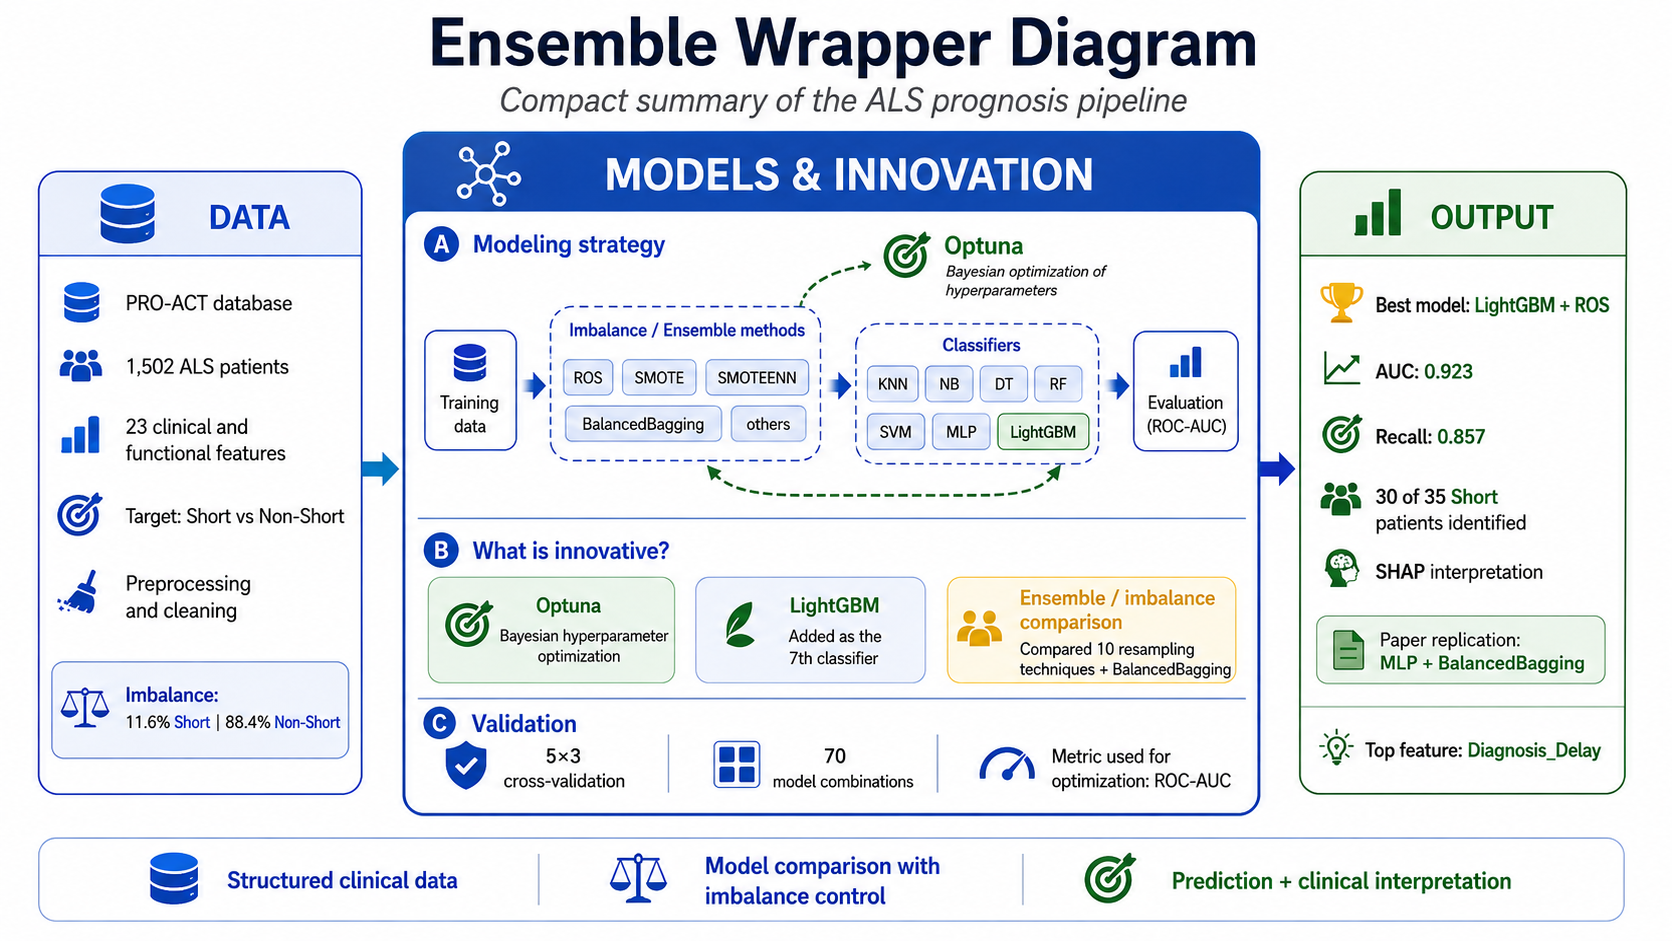
\includegraphics[width=\linewidth]{figures/ensemble_wrapper.png}
  \caption{Study overview. \textit{Left:} PRO-ACT dataset characteristics and
    class distribution (11.6\% Short Survivors vs.\ 88.4\% Standard Survival).
    \textit{Centre:} experimental pipeline comprising imbalance-handling
    strategies, seven classifiers, and Bayesian hyperparameter optimisation
    (Optuna), validated via 5$\times$3 repeated stratified cross-validation
    across 70 model combinations. \textit{Right:} best model results
    (LightGBM\,+\,ROS: AUC\,=\,0.923, Recall\,=\,0.857) and replication
    finding (MLP\,+\,BalancedBagging).}
  \label{fig:overview}
\end{figure}
\end{comment}

% ==========================================================================
\section{Related Work}
\label{sec:related}
% ==========================================================================

\subsection{Machine Learning for ALS Prognosis}

ML approaches to ALS progression modelling have multiplied over the past decade,
with the PRO-ACT database serving as the shared benchmark for most of them. Early
crowdsourced efforts by K\"{u}ffner et al.~\cite{kueffner2019} showed that
ensemble models could predict ALSFRS-R slope at accuracy levels competitive with
specialist clinical benchmarks. More recent work has explored deep learning
architectures for continuous trajectory modelling, including recurrent and
multi-task networks applied to longitudinal ALSFRS-R
data~\cite{Pancotti2022,Qin2025}. Ramamoorthy et al.~\cite{Ramamoorthy2022}
proposed a Gaussian-process framework for identifying progression patterns from
sparse longitudinal records.

At the level of binary survival classification, Halbersberg and
Lerner~\cite{Halbersberg2023} compared several ML methods for ALS stratification,
finding that ensemble-based approaches consistently outperformed individual
classifiers. Anani et al.~\cite{Anani2023} combined feature selection with
interpretable modelling to isolate the most prognostically informative variables.
Papaiz et al.~\cite{Papaiz2022}, in a systematic review, pinpointed class
imbalance and limited dataset size as the two recurring obstacles to reliable ALS
prognosis. Wang et al.~\cite{Wang2025} surveyed explainable AI across
neurodegenerative diseases, noting the widening gap between model complexity and
clinical interpretability.

\subsection{Imbalance-Aware Learning and Ensemble Methods}

Correcting for class imbalance in medical classification is a well-studied problem. Resampling strategies include synthetic oversampling methods like
SMOTE~\cite{chawla2002smote}, BorderlineSMOTE, and ADASYN, as well as
undersampling methods such as Random Undersampling (RUS) and NearMiss. Hybrid
approaches (SMOTETomek and SMOTEENN) combine both paradigms to remove noisy
boundary samples alongside oversampling. The \texttt{imbalanced-learn}
library~\cite{lemaitre2017} provides scikit-learn-compatible implementations of
all these strategies, including BalancedBagging, which applies random
undersampling internally within each bootstrap estimator. Which technique works
best is highly problem-dependent; there is no universally superior strategy,
which is why systematic cross-validated comparison across multiple classifiers
remains the most defensible selection approach.

\subsection{Bayesian Hyperparameter Optimisation}

Grid search, as used in the reference study, evaluates hyperparameters on a fixed
predefined lattice, which scales poorly with the number of parameters and may
miss near-optimal configurations that lie between grid points. Bayesian
optimisation addresses this by building a probabilistic surrogate model of the
objective function and directing new evaluations towards promising regions.
Optuna~\cite{optuna2019}, built around the Tree-structured Parzen Estimator
(TPE), is widely used for this purpose; its define-by-run API and
automatic trial pruning make it practical for large search spaces.

\subsection{Explainability in Clinical ML}

SHAP (SHapley Additive exPlanations)~\cite{lundberg2017shap} frames feature
attribution as a cooperative game: each feature is credited for its marginal
contribution to a prediction, averaged across all possible feature orderings.
For tree-based models, TreeSHAP~\cite{lundberg2020treeshap} computes these values
exactly in polynomial time. KernelSHAP extends the approach to architectures such
as MLPs via sampling-based approximation, at higher computational cost. Applied
to ALS prognosis~\cite{Anani2023}, SHAP has consistently ranked functional decline
metrics as the dominant predictors, consistent with clinical observation.

% ==========================================================================
\section{Methodology}
\label{sec:methodology}
% ==========================================================================

Figure~\ref{fig:workflow} provides an overview of the complete experimental
pipeline described in this section.
\clearpage
\begin{figure}[ht!]
\centering
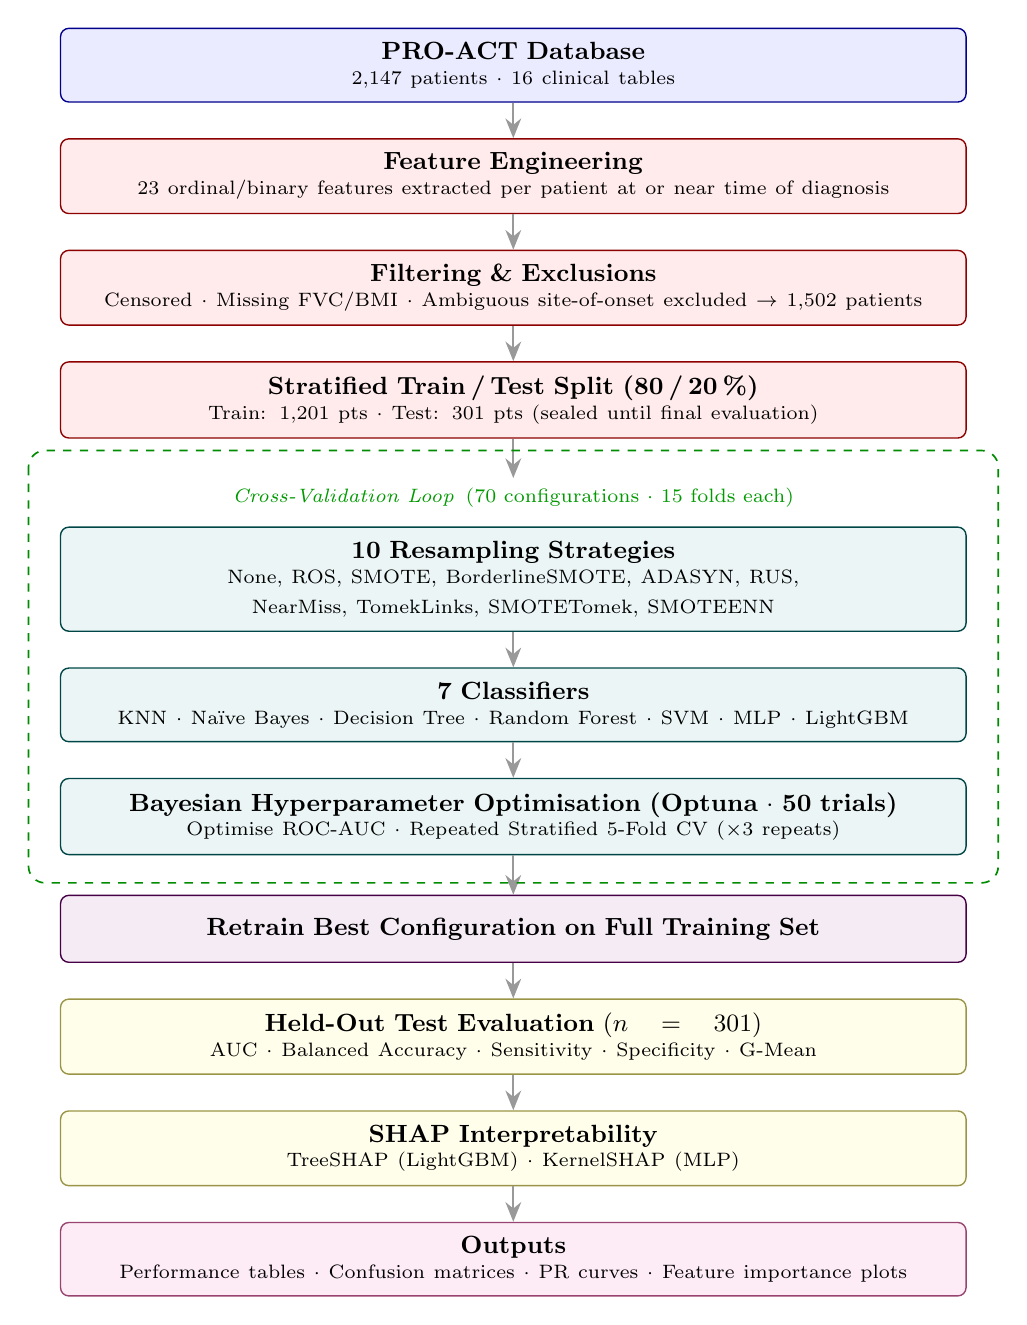
\begin{tikzpicture}[
  sbox/.style={
    rectangle, rounded corners=3pt, draw=#1!55!black, fill=#1!8,
    minimum width=11.5cm, minimum height=0.85cm,
    text centered, font=\small, text width=11cm, inner sep=5pt,
    line width=0.5pt
  },
  sbox/.default={blue},
  arr/.style={-{Stealth[length=2.5mm, width=2mm]}, draw=black!40, line width=0.7pt},
  node distance=0.45cm
]

% === Data source ===
\node[sbox=blue] (s1) {
  \textbf{PRO-ACT Database}\\[-2pt]
  {\scriptsize 2{,}147 patients $\cdot$ 16 clinical tables}
};

% === Preprocessing ===
\node[sbox=red, below=of s1] (s2) {
  \textbf{Feature Engineering}\\[-2pt]
  {\scriptsize 23 ordinal/binary features extracted per patient at or near time of diagnosis}
};

\node[sbox=red, below=of s2] (s3) {
  \textbf{Filtering \& Exclusions}\\[-2pt]
  {\scriptsize Censored $\cdot$ Missing FVC/BMI $\cdot$ Ambiguous site-of-onset
    excluded $\rightarrow$ 1{,}502 patients}
};

\node[sbox=red, below=of s3] (s4) {
  \textbf{Stratified Train\,/\,Test Split (80\,/\,20\,\%)}\\[-2pt]
  {\scriptsize Train: 1{,}201 pts $\cdot$ Test: 301 pts (sealed until final evaluation)}
};

% === CV label (same width as sbox → symmetric bounding box) ===
\node[minimum width=11.5cm, align=center,
      font=\scriptsize\itshape, text=green!60!black,
      below=0.5cm of s4] (cvlabel)
  {Cross-Validation Loop\enspace\textnormal{(70 configurations $\cdot$ 15 folds each)}};

% === CV loop nodes ===
\node[sbox=teal, below=0.12cm of cvlabel] (s5) {
  \textbf{10 Resampling Strategies}\\[-2pt]
  {\scriptsize None, ROS, SMOTE, BorderlineSMOTE, ADASYN,
    RUS, NearMiss, TomekLinks, SMOTETomek, SMOTEENN}
};

\node[sbox=teal, below=of s5] (s6) {
  \textbf{7 Classifiers}\\[-2pt]
  {\scriptsize KNN $\cdot$ Na\"{i}ve Bayes $\cdot$ Decision Tree $\cdot$
    Random Forest $\cdot$ SVM $\cdot$ MLP $\cdot$ LightGBM}
};

\node[sbox=teal, below=of s6] (s7) {
  \textbf{Bayesian Hyperparameter Optimisation (Optuna $\cdot$ 50 trials)}\\[-2pt]
  {\scriptsize Optimise ROC-AUC $\cdot$
    Repeated Stratified 5-Fold CV ($\times$3 repeats)}
};

% === Post-CV ===
\node[sbox=violet, below=0.5cm of s7] (s8) {
  \textbf{Retrain Best Configuration on Full Training Set}
};

% === Evaluation ===
\node[sbox=yellow, below=of s8] (s9) {
  \textbf{Held-Out Test Evaluation} ($n = 301$)\\[-2pt]
  {\scriptsize AUC $\cdot$ Balanced Accuracy $\cdot$
    Sensitivity $\cdot$ Specificity $\cdot$ G-Mean}
};

\node[sbox=yellow, below=of s9] (s10) {
  \textbf{SHAP Interpretability}\\[-2pt]
  {\scriptsize TreeSHAP (LightGBM) $\cdot$ KernelSHAP (MLP)}
};

% === Output ===
\node[sbox=magenta, below=of s10] (s11) {
  \textbf{Outputs}\\[-2pt]
  {\scriptsize Performance tables $\cdot$ Confusion matrices $\cdot$
    PR curves $\cdot$ Feature importance plots}
};

% === ARROWS ===
\draw[arr] (s1)  -- (s2);
\draw[arr] (s2)  -- (s3);
\draw[arr] (s3)  -- (s4);
\draw[arr] (s4.south) -- (cvlabel.north);
\draw[arr] (s5)  -- (s6);
\draw[arr] (s6)  -- (s7);
\draw[arr] (s7.south) -- (s8.north);
\draw[arr] (s8)  -- (s9);
\draw[arr] (s9)  -- (s10);
\draw[arr] (s10) -- (s11);

% === CV dashed border (drawn via coordinates — no fit node) ===
\draw[green!55!black, dashed, rounded corners=6pt, line width=0.6pt]
  ([shift={(-0.4cm, 0.35cm)}]cvlabel.north west)
  rectangle
  ([shift={(0.4cm,-0.35cm)}]s7.south east);

\end{tikzpicture}
\caption{Overview of the experimental pipeline. The dashed border delimits
  the cross-validation loop, which was applied exclusively to the training
  partition. The test set remained sealed until all model selection and
  hyperparameter optimisation had been completed.}
\label{fig:workflow}
\end{figure}


\subsection{Dataset Overview}

The PRO-ACT database~\cite{PROACT} contains longitudinal clinical records from
ALS patients enrolled across multiple controlled trials, covering ALSFRS-R
assessments, vital signs, forced vital capacity (FVC), medication history, and
demographic data. The publicly available extract examined here comprises
2,147 patient records across 16 clinical tables prior to any filtering.
Following the feature engineering protocol of
Papaiz et al.~\cite{Papaiz2024}, we extracted 23 categorical and ordinal features
representing each patient's clinical status at or near the time of diagnosis.

Throughout this paper, patients who died within 24 months of symptom onset are
termed \textbf{Short Survivors}; those who died after 24 months or were alive
beyond that point are termed \textbf{Standard Survival} patients. The binary target variable is defined
accordingly: Short Survivor (death $\leq$ 24 months from symptom onset) versus
Standard Survival (death $>$ 24 months, or alive beyond 24 months).
Patients alive at the time of their last observation but without
24 months of confirmed follow-up were treated as censored and excluded, consistent
with the reference study. Patients missing site-of-onset records were also excluded.

Table~\ref{tab:dataset} compares the resulting dataset with the one reported in
the reference study. Our cohort comprises 1,502 patients, 23.6\% fewer than the
original, primarily because the publicly available PRO-ACT extract examined here
contains a substantially higher proportion of missing FVC records (62.3\% after
survival and site filtering) and sparser height data required for BMI derivation.
The imbalance ratio rises correspondingly (7.6 versus 6.9).

\begin{table}[ht!]
  \centering
  \caption{Dataset comparison between the reference study~\protect\cite{Papaiz2024}
    and this work.}
  \label{tab:dataset}
  \begin{tabular}{lcc}
    \toprule
    \textbf{Metric} & \textbf{Reference Study} & \textbf{This Work} \\
    \midrule
    Total patients   & 1,967          & 1,502          \\
    Short Survivors (\%)    & 13.0\% (256)   & 11.6\% (174)   \\
    Standard Survival (\%)  & 87.0\% (1,711) & 88.4\% (1,328) \\
    Imbalance ratio  & 6.9            & 7.6            \\
    Features         & 23             & 23             \\
    \bottomrule
  \end{tabular}
\end{table}

\subsection{Data Preprocessing}

Preprocessing mirrored the reference study's pipeline. Binary features---sex,
site of onset, Riluzole use, and gastrostomy---were encoded as 0/1 indicators.
Age at onset was discretised into five ordinal groups ($\leq$39, 40--49, 50--59,
60--69, $\geq$70). Diagnostic delay was categorised as short ($\leq$8 months),
average (9--18 months), or long ($\geq$19 months), a proxy for pre-diagnostic
disease tempo. FVC at diagnosis was classified as abnormal ($<$80\% predicted) or
normal. BMI was derived from body weight and height measurements closest to the
diagnosis visit and encoded into four standard categories. ALSFRS-R functional
decline slopes for each of the ten subscores (Q1--Q10) were
computed as $(4 - \text{score}) / \text{months from symptom onset}$ at the
assessment visit closest in time to each patient's diagnosis date, following the
formulation of the reference study~\cite{Papaiz2024}. Where no pre-diagnosis
assessment was available, the nearest available visit was used instead; this
introduces a limited risk of post-diagnosis information being incorporated for a
subset of patients, a limitation discussed further in Section~\ref{sec:discussion}.
Slopes were binned as slow ($<$0.05), average (0.05--0.14), or rapid
($\geq$0.14 points per month). Disease regions involved (bulbar, upper limb,
lower limb, respiratory) were derived from ALSFRS-R subscores at the same visit.

\subsection{Data Partitioning}

The dataset was split 80/20 into training ($n = 1{,}201$; 139 Short Survivors,
1,062 Standard Survival) and test ($n = 301$; 35 Short Survivors, 266 Standard
Survival) partitions using stratified sampling (random seed 42). The test set was
sealed until all model selection and hyperparameter optimisation had been completed.

\subsection{Experimental Setup}
\label{subsec:setup}

\paragraph{Classifiers.}
Seven classifiers were evaluated: K-Nearest Neighbours (KNN), Naïve Bayes (NB),
Decision Tree (DT), Random Forest (RF), Support Vector Machine (SVM),
Multi-Layer Perceptron (MLP), and LightGBM~\cite{ke2017lightgbm}. The first six
correspond directly to those used in the reference study; LightGBM is the primary
addition to the original six.

The best-performing MLP configuration, identified by Optuna, consists of a
single hidden layer with 172 neurons (\texttt{tanh} activation), an input
layer of 23 units (one per feature), and a single output unit with logistic
activation producing the probability of Short Survivor class membership.
Training used the Adam optimiser with an adaptive learning rate schedule and
L2 regularisation ($\alpha \approx 0.061$), for a maximum of 1{,}000
iterations without early stopping.
Classification used the default decision threshold of 0.5.

\begin{figure}[ht!]
\centering
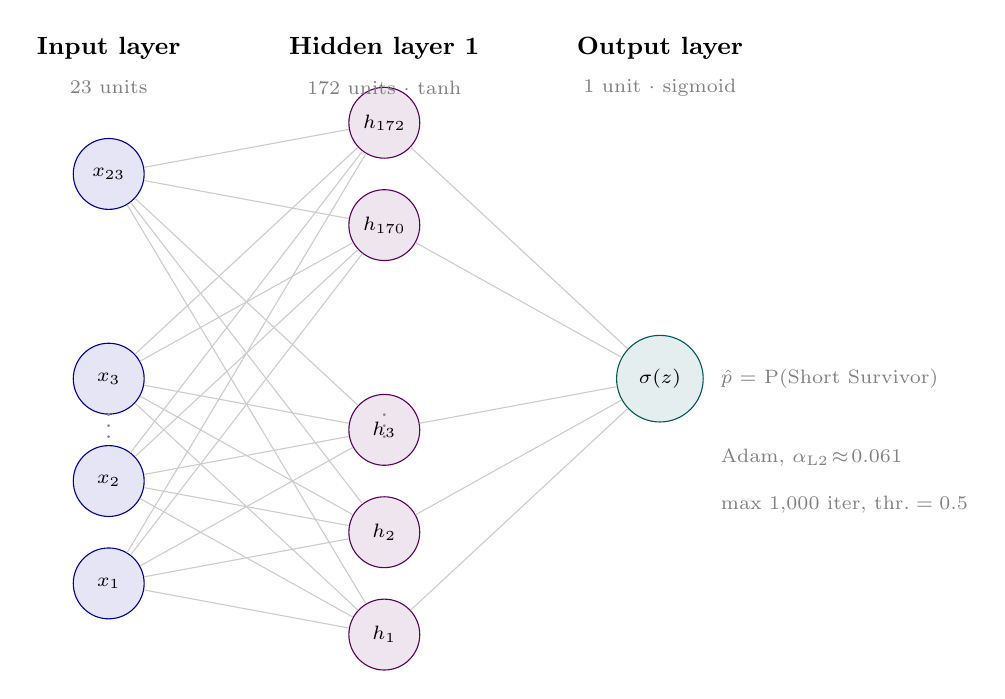
\begin{tikzpicture}[
  neuron/.style={circle, draw=#1, fill=#1!10, minimum size=9mm,
                 inner sep=0pt, font=\scriptsize},
  layer/.style={font=\small\bfseries},
  sublabel/.style={font=\scriptsize, text=gray},
  conn/.style={draw=gray!40, line width=0.4pt},
  >=stealth
]

\def\layerA{1.0}  % x of input layer
\def\layerB{4.5}  % x of hidden layer
\def\layerC{8.0}  % x of output layer

% --- Input layer (5 shown + implicit ellipsis) ---
\foreach \i/\lbl in {1/$x_1$, 2/$x_2$, 3/$x_3$, 5/$x_{23}$}{
  \pgfmathsetmacro\ypos{(\i-3)*1.3}
  \node[neuron=blue!60!black] (I\i) at (\layerA,\ypos) {\lbl};
}
% Ellipsis between x3 and x23
\node[font=\small, text=gray] at (\layerA, -0.5) {$\vdots$};

% --- Hidden layer (6 shown + ellipsis) ---
\foreach \i/\lbl in {1/$h_1$, 2/$h_2$, 3/$h_3$, 5/$h_{170}$, 6/$h_{172}$}{
  \pgfmathsetmacro\ypos{(\i-3.5)*1.3}
  \node[neuron=violet!70!black] (H\i) at (\layerB,\ypos) {\lbl};
}
\node[font=\small, text=gray] at (\layerB, -0.5) {$\vdots$};

% --- Output layer ---
\node[neuron=teal!70!black, minimum size=11mm] (O) at (\layerC, 0)
  {$\sigma(z)$};

% --- Connections (sampled, not exhaustive) ---
\foreach \src in {I1,I2,I3,I5}{
  \foreach \dst in {H1,H2,H3,H5,H6}{
    \draw[conn] (\src) -- (\dst);
  }
}
\foreach \src in {H1,H2,H3,H5,H6}{
  \draw[conn] (\src) -- (O);
}

% --- Layer header labels ---
\node[layer] at (\layerA, 4.2)  {Input layer};
\node[sublabel] at (\layerA, 3.7) {23 units};

\node[layer] at (\layerB, 4.2)  {Hidden layer 1};
\node[sublabel] at (\layerB, 3.7) {172 units $\cdot$ tanh};

\node[layer] at (\layerC, 4.2)  {Output layer};
\node[sublabel] at (\layerC, 3.7) {1 unit $\cdot$ sigmoid};

% --- Output annotation ---
\node[font=\scriptsize, align=left, text=gray, anchor=west]
  at (\layerC+0.65, 0.0) {$\hat{p}$ = P(Short Survivor)};

% --- Training note ---
\node[font=\scriptsize, align=left, text=gray, anchor=west]
  at (\layerC+0.65, -1.0)
  {Adam, $\alpha_{\text{L2}}\!\approx\!0.061$};
\node[font=\scriptsize, align=left, text=gray, anchor=west]
  at (\layerC+0.65, -1.6)
  {max 1{,}000 iter, thr.\;$=0.5$};

\end{tikzpicture}
\caption{Architecture of the best-performing MLP configuration identified
  by Optuna. The network comprises an input layer of 23 units (one per
  clinical feature), a single hidden layer of 172 neurons with tanh
  activation, and a single output unit with logistic (sigmoid) activation
  producing $\hat{p} =$ P(Short Survivor). Training used the Adam
  optimiser with L2 regularisation ($\alpha \approx 0.061$) for a
  maximum of 1{,}000 iterations. Classification was applied at the
  default decision threshold of 0.5.}
\label{fig:mlp_arch}
\end{figure}


\paragraph{Imbalance-handling strategies.}
Ten class-imbalance correction strategies were evaluated: no correction (None),
Random Oversampling (ROS), SMOTE~\cite{chawla2002smote}, Borderline-SMOTE,
ADASYN, Random Undersampling (RUS), NearMiss, TomekLinks, SMOTETomek, and
SMOTEENN, yielding 70 classifier--technique combinations in total.
\textbf{Critically, all resampling operations were applied exclusively to the
training fold of each cross-validation iteration, after the fold split and before
classifier fitting; the validation fold and the held-out test set were never
touched by any resampling procedure.} Cross-validation estimates and final test
performance therefore both reflect the natural class distribution (11.6\% Short
Survivors), with no leakage from held-out samples into the resampled training
distribution.

\paragraph{Hyperparameter optimisation.}
Replacing the original grid search, we employed Optuna~\cite{optuna2019} with the
TPE sampler for each of the 70 combinations, running 50 evaluation trials per
combination. ROC-AUC was used as the optimisation criterion, averaged over
cross-validation folds, matching the reference study's evaluation metric exactly.
Optimising for the same criterion means any divergence between cross-validation
AUC and held-out minority-class performance can be attributed to properties of the
criterion itself, not to differences in model selection procedure.
Section~\ref{sec:results} shows the consequence directly.
Classifier-specific hyperparameter
search spaces were defined to cover a broad range of architectures (e.g.\ number
of layers and neurons for MLP; number of estimators and tree depth for RF and
LightGBM).

\paragraph{Cross-validation.}
Model selection was conducted using Repeated Stratified $K$-Fold cross-validation
with $K = 5$ and 3 repeats (15 evaluations per configuration), applied
exclusively to the training set.

\paragraph{BalancedBagging replication.}
To directly replicate the reference study, all seven classifiers were additionally
evaluated in two scenarios using the same cross-validation protocol: (i) a
single-model baseline with no imbalance correction, and (ii) wrapped inside a
BalancedBagging ensemble~\cite{lemaitre2017} with ten estimators and random
undersampling applied within each bootstrap iteration.

\paragraph{Statistical validation.}
Per-fold balanced accuracy scores from the 15 cross-validation folds were compared
between the single-model and BalancedBagging configurations for each classifier
using the Wilcoxon signed-rank test~\cite{wilcoxon1945}. Family-wise error rate
inflation across the seven simultaneous comparisons was controlled by applying
Bonferroni correction (corrected significance threshold
$\alpha_c = 0.05 / 7 \approx 0.007$).

\paragraph{SHAP interpretability.}
Feature importance was assessed using TreeSHAP~\cite{lundberg2020treeshap} for
LightGBM and KernelSHAP~\cite{lundberg2017shap} for the MLP (100 background
samples, 200 evaluation samples per instance). SHAP values were computed on the
held-out test set for both models after final retraining on the full training set.

\paragraph{Evaluation metrics.}
Models were assessed using ROC-AUC, balanced accuracy, sensitivity (recall for the
Short Survivor class), specificity, and geometric mean (G-Mean). Missing a Short
Survivor is the worst-case error; sensitivity is therefore the primary metric
throughout.

To investigate the effect of the decision boundary, three alternative thresholds
were derived per classifier from out-of-fold (OOF) cross-validation predictions---never
from the held-out test set---using (i)~Youden's J statistic~\cite{youden1950}, (ii) the
highest threshold achieving sensitivity $\geq 0.90$, and (iii) the threshold maximising
minority-class F1 score. These thresholds were subsequently applied to the test set
and evaluated alongside the default 0.50 boundary; full results are reported in
Section~\ref{subsec:threshold}.

Given the small number of Short Survivors in the test set ($n = 35$), point
estimates shift by 2.86 percentage points per patient. Bootstrap 95\% percentile
confidence intervals (2\,000 resamples, \texttt{random\_state}$=42$) were therefore
computed for all held-out metrics. Bootstrap samples containing no Short Survivors
were excluded from sensitivity and G-Mean calculations; the count per classifier is
reported alongside each point estimate in Table~\ref{tab:test}.

% ==========================================================================
\section{Results}
\label{sec:results}
% ==========================================================================

\subsection{Cross-Validation Performance}

Table~\ref{tab:cv} shows, for each classifier, the highest-AUC configuration
found across 70 Optuna-optimised combinations, averaged over 15 cross-validation
folds.

\begin{table}[ht!]
  \centering
  \caption{Best cross-validation results per classifier (Optuna, 70 combinations,
    15-fold repeated CV). Sensitivity and specificity refer to the Short Survivor
    (minority) class. G-Mean $= \sqrt{\text{Sensitivity} \times \text{Specificity}}$.}
  \label{tab:cv}
  \resizebox{\linewidth}{!}{%
  \begin{tabular}{llcccc}
    \toprule
    \textbf{Classifier} & \textbf{Best Technique} & \textbf{AUC}
      & \textbf{Sensitivity} & \textbf{Specificity} & \textbf{G-Mean} \\
    \midrule
    MLP           & None       & 0.915 & 0.427 & 0.969 & 0.641 \\
    LightGBM      & ROS        & 0.914 & 0.780 & 0.864 & 0.819 \\
    SVM           & SMOTEENN   & 0.911 & 0.904 & 0.784 & 0.842 \\
    Random Forest & None       & 0.906 & 0.276 & 0.983 & 0.517 \\
    Naïve Bayes   & None       & 0.891 & 0.727 & 0.867 & 0.793 \\
    KNN           & RUS        & 0.880 & 0.767 & 0.831 & 0.797 \\
    Decision Tree & TomekLinks & 0.861 & 0.413 & 0.948 & 0.621 \\
    \bottomrule
  \end{tabular}%
  }
\end{table}

The MLP achieves the highest cross-validation AUC (0.915) but at the expense of
low minority-class sensitivity (0.427). The Optuna configuration behind this result is suggestive: the best MLP carries a comparatively strong L2 penalty
($\alpha = 0.061$), roughly five times larger than the values found for the same
architecture under any resampling strategy. This may indicate that regularisation
is suppressing the model's tendency to assign uniformly high scores to Standard Survival patients,
improving probability ranking (and therefore AUC) without pushing minority-class
scores above the 0.5 decision boundary. The result is consistent with a model
that has traded sensitivity for ranking fidelity in cross-validation, a pattern
that becomes fully visible at test time.
LightGBM with Random Oversampling sits one AUC point behind (0.914) but delivers
sensitivity of 0.780 and G-Mean of 0.819. Three classifiers---MLP, Random Forest,
and Naïve Bayes---reach their best AUC with no imbalance correction at all.
For MLP and Random Forest, that high AUC coexists with poor sensitivity. The
held-out test will make this gap impossible to ignore.

\subsection{Held-Out Test Set Evaluation}

After model selection was finalised on the training set, each classifier was
retrained on the full training partition and evaluated on the sealed test set
(35 Short Survivors, 266 Standard Survival patients). Results appear in
Table~\ref{tab:test}.

\begin{table}[ht!]
  \centering
  \caption{Held-out test set performance for each classifier under its best
    cross-validation configuration. Each cell shows the point estimate with the
    bootstrap 95\% percentile confidence interval in parentheses
    (2\,000 resamples; no bootstrap sample contained zero Short Survivors).
    Bold indicates the best point estimate per metric.
    With 35 Short Survivors, one patient $= 2.86$\,pp; the sensitivity CIs of
    LightGBM+ROS and SVM+SMOTEENN overlap, indicating the one-patient difference
    is not statistically distinguishable.}
  \label{tab:test}
  \resizebox{\linewidth}{!}{%
  \begin{tabular}{llccccc}
    \toprule
    \textbf{Classifier} & \textbf{Technique} & \textbf{AUC}
      & \textbf{Bal.\ Acc.} & \textbf{Sensitivity} & \textbf{Specificity}
      & \textbf{G-Mean} \\
    \midrule
    LightGBM
      & ROS
      & \textbf{0.923} {\small(0.868--0.966)}
      & \textbf{0.844} {\small(0.774--0.903)}
      & 0.857 {\small(0.724--0.967)}
      & 0.831 {\small(0.784--0.876)}
      & \textbf{0.844} {\small(0.772--0.902)} \\
    Random Forest
      & None
      & 0.919 {\small(0.868--0.958)}
      & 0.623 {\small(0.551--0.700)}
      & 0.257 {\small(0.114--0.412)}
      & 0.989 {\small(0.974--1.000)}
      & 0.504 {\small(0.337--0.638)} \\
    MLP
      & None
      & 0.918 {\small(0.874--0.955)}
      & 0.514 {\small(0.500--0.550)}
      & 0.029 {\small(0.000--0.100)}
      & \textbf{1.000} {\small(1.000--1.000)}
      & 0.169 {\small(0.000--0.316)} \\
    SVM
      & SMOTEENN
      & 0.908 {\small(0.863--0.946)}
      & 0.826 {\small(0.759--0.880)}
      & \textbf{0.886} {\small(0.765--0.975)}
      & 0.767 {\small(0.714--0.821)}
      & 0.824 {\small(0.758--0.875)} \\
    Naïve Bayes
      & None
      & 0.889 {\small(0.834--0.937)}
      & 0.774 {\small(0.694--0.847)}
      & 0.714 {\small(0.556--0.853)}
      & 0.835 {\small(0.789--0.881)}
      & 0.772 {\small(0.682--0.847)} \\
    KNN
      & RUS
      & 0.886 {\small(0.834--0.933)}
      & 0.812 {\small(0.738--0.879)}
      & 0.800 {\small(0.655--0.925)}
      & 0.823 {\small(0.779--0.870)}
      & 0.812 {\small(0.735--0.878)} \\
    Decision Tree
      & TomekLinks
      & 0.874 {\small(0.805--0.931)}
      & 0.628 {\small(0.555--0.706)}
      & 0.286 {\small(0.136--0.440)}
      & 0.970 {\small(0.948--0.989)}
      & 0.526 {\small(0.364--0.654)} \\
    \bottomrule
  \end{tabular}%
  }
\end{table}

The MLP detected one Short Survivor. One, out of 35.
Sensitivity is 0.029. Balanced accuracy is 0.514 (essentially a coin flip).
Specificity of 1.000 is not a strength; it means the model labelled 34 of 35
Short Survivors as Standard Survival, as shown in Figure~\ref{fig:cm}.
Yet its test AUC is 0.918, the third highest. It can rank patients by risk;
it cannot classify them at the default threshold. Figures~\ref{fig:cvtest}
and~\ref{fig:decoupling} show this gap across all seven classifiers.
The name for it is AUC--sensitivity decoupling: a model that correctly orders
probabilities on average can still compress every minority-class score below
0.5, making Short Survivors invisible at the operating point. The
precision-recall curves in Figure~\ref{fig:pr} confirm this. Despite an average
precision of 0.669, the MLP's minority-class probabilities cluster below
the decision threshold for nearly all patients, with only one crossing 0.5.

LightGBM with Random Oversampling identified 30 of 35 Short Survivors
(sensitivity 0.857, 95\%\,CI [0.724,\,0.967]; specificity 0.831; AUC 0.923).
SVM with SMOTEENN caught 31 of 35 (sensitivity 0.886, 95\%\,CI
[0.765,\,0.975]), but at lower specificity (0.767) and AUC (0.909). The
sensitivity confidence intervals of these two models overlap substantially
(Table~\ref{tab:test}): the one-patient difference is not statistically
distinguishable given the 35-patient minority class. Both models serve
different use cases---SVM+SMOTEENN when missing a Short Survivor is the
worst outcome; LightGBM+ROS when overall balance across all metrics
matters---but neither is decisively superior by sensitivity alone.

\begin{figure}[ht!]
  \centering
  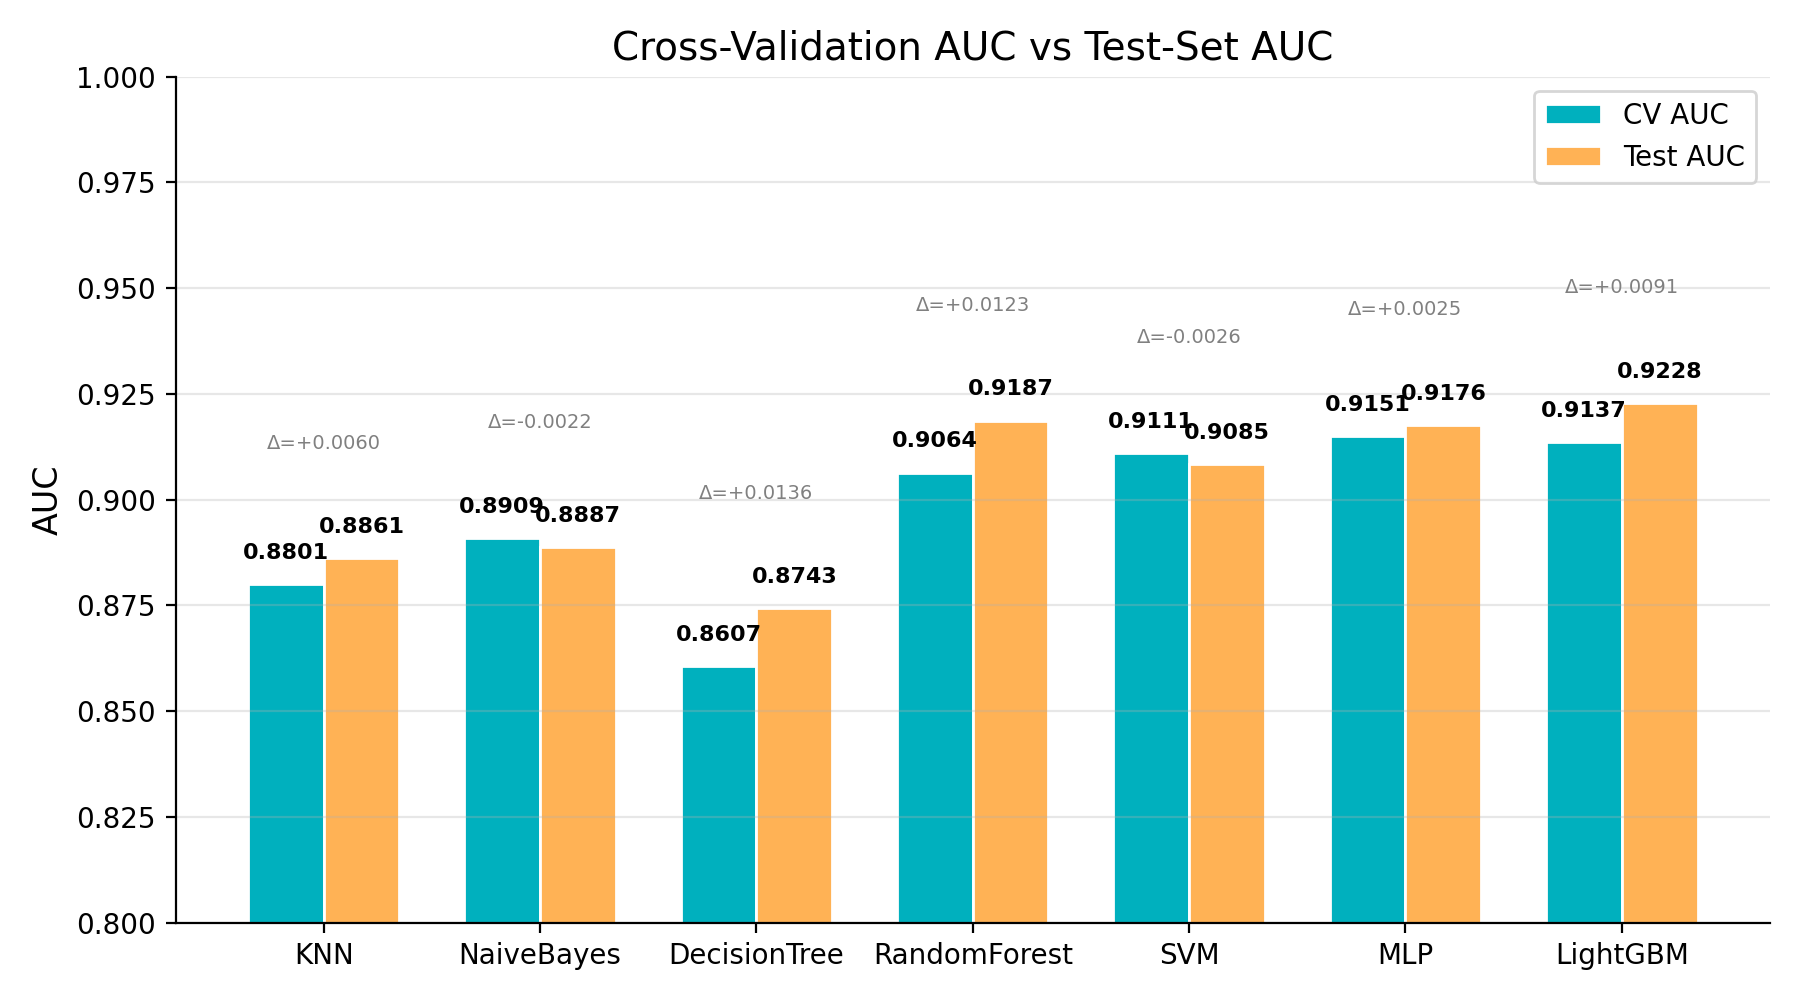
\includegraphics[width=0.95\linewidth]{figures/step6_cv_vs_test.png}
  \caption{Cross-validation AUC versus held-out test AUC for all seven
    classifiers. The MLP ranks first in CV AUC (0.915) yet achieves near-chance
    sensitivity on the test set (0.029), illustrating the AUC--sensitivity
    decoupling under severe class imbalance.}
  \label{fig:cvtest}
  \vspace{0.8em}
  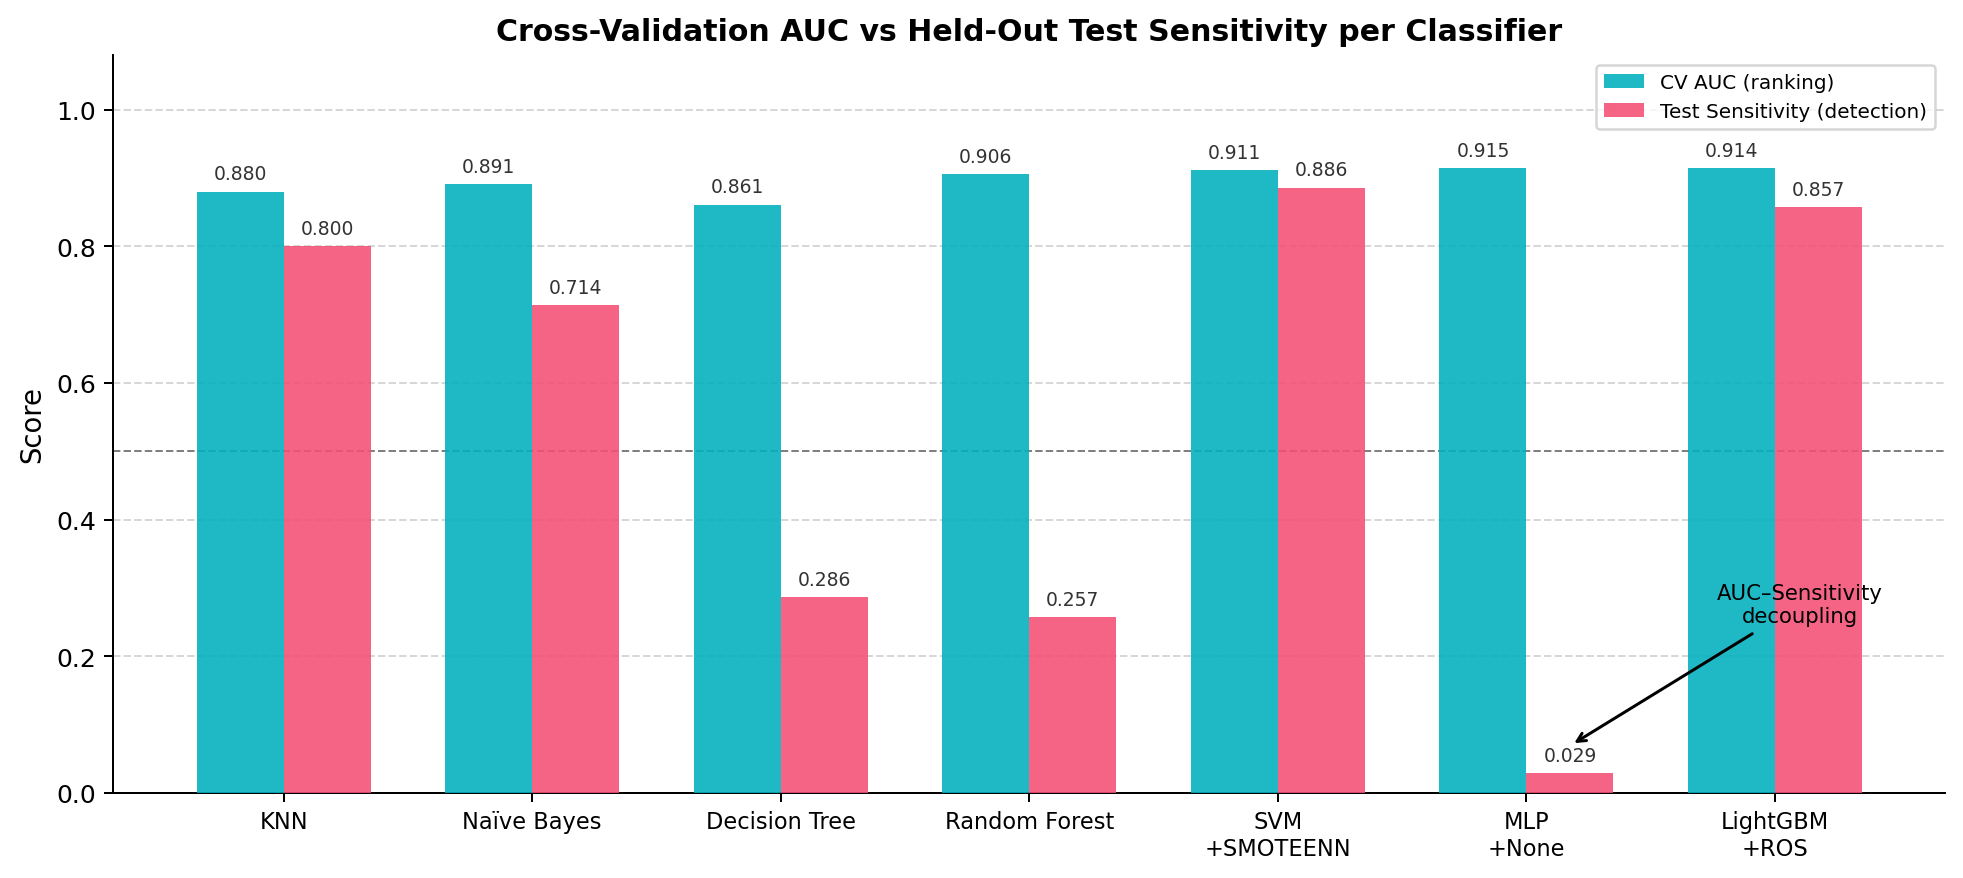
\includegraphics[width=0.95\linewidth]{figures/fig_auc_sensitivity_decoupling.png}
  \caption{Cross-validation AUC versus held-out test sensitivity for all seven
    classifiers under their best configurations. The MLP achieves the highest CV
    AUC (0.915) yet collapses to near-zero sensitivity (0.029) on the test set,
    while LightGBM+ROS and SVM+SMOTEENN maintain sensitivity above 0.85 with
    competitive AUC values.}
  \label{fig:decoupling}
\end{figure}

\clearpage
\begin{figure}[t!]
  \centering
  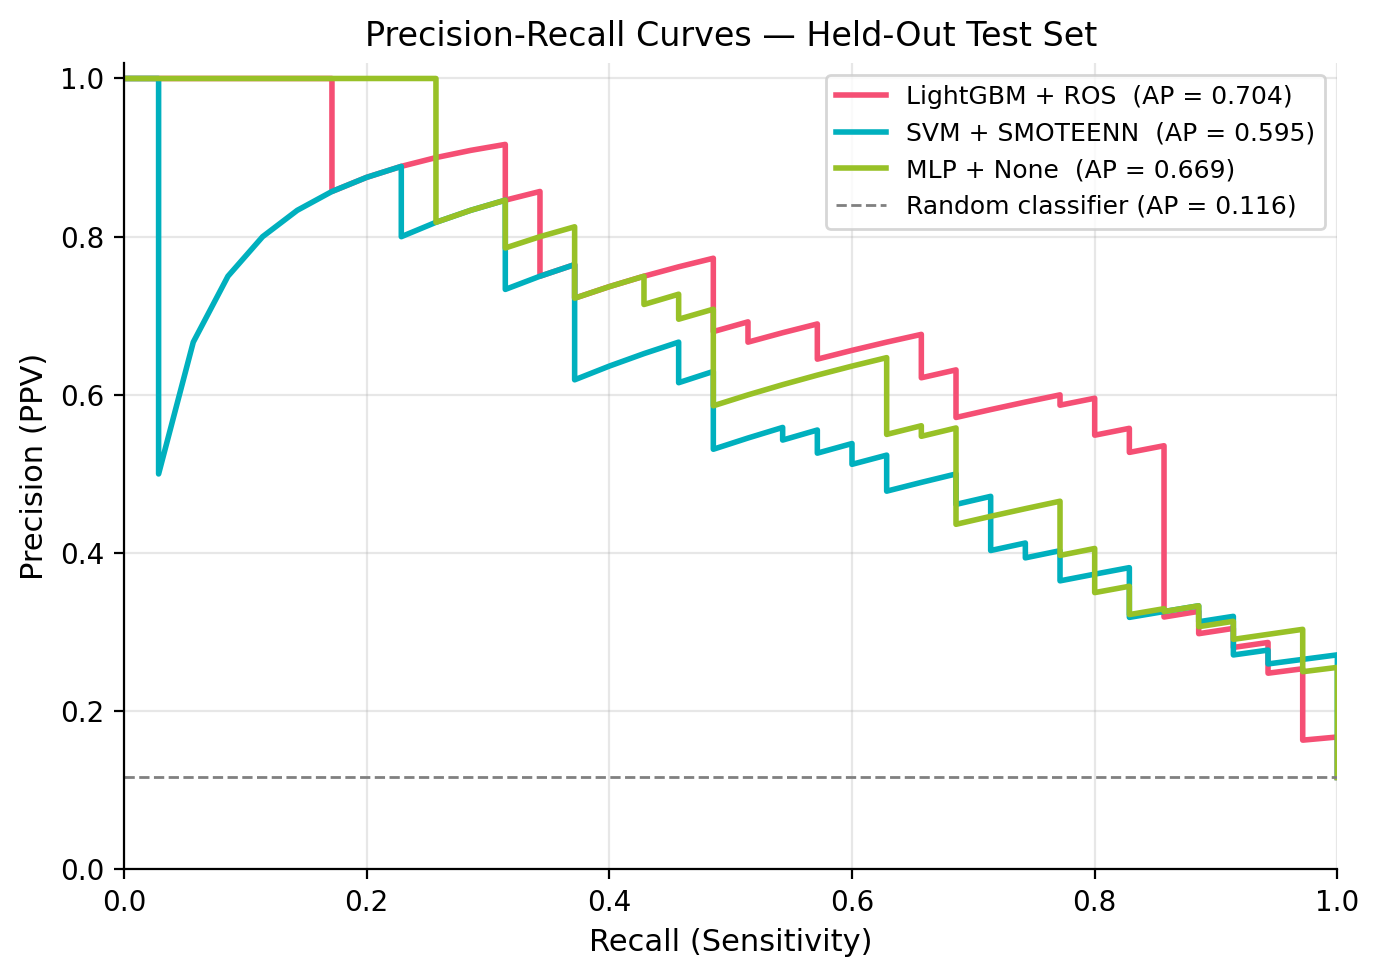
\includegraphics[width=0.95\linewidth]{figures/fig_pr_curves.png}
  \caption{Precision-recall curves on the held-out test set for the three
    highlighted classifiers. Despite a competitive AP (LightGBM+ROS: 0.704,
    MLP: 0.669, SVM+SMOTEENN: 0.595), the MLP's minority-class probabilities
    cluster below the default threshold, collapsing to near-zero sensitivity
    at the operating point. The dashed line marks the random-classifier baseline
    (AP$\,{=}\,$prevalence $\approx$ 0.116).}
  \label{fig:pr}
\end{figure}

\begin{figure}[ht!]
  \centering
  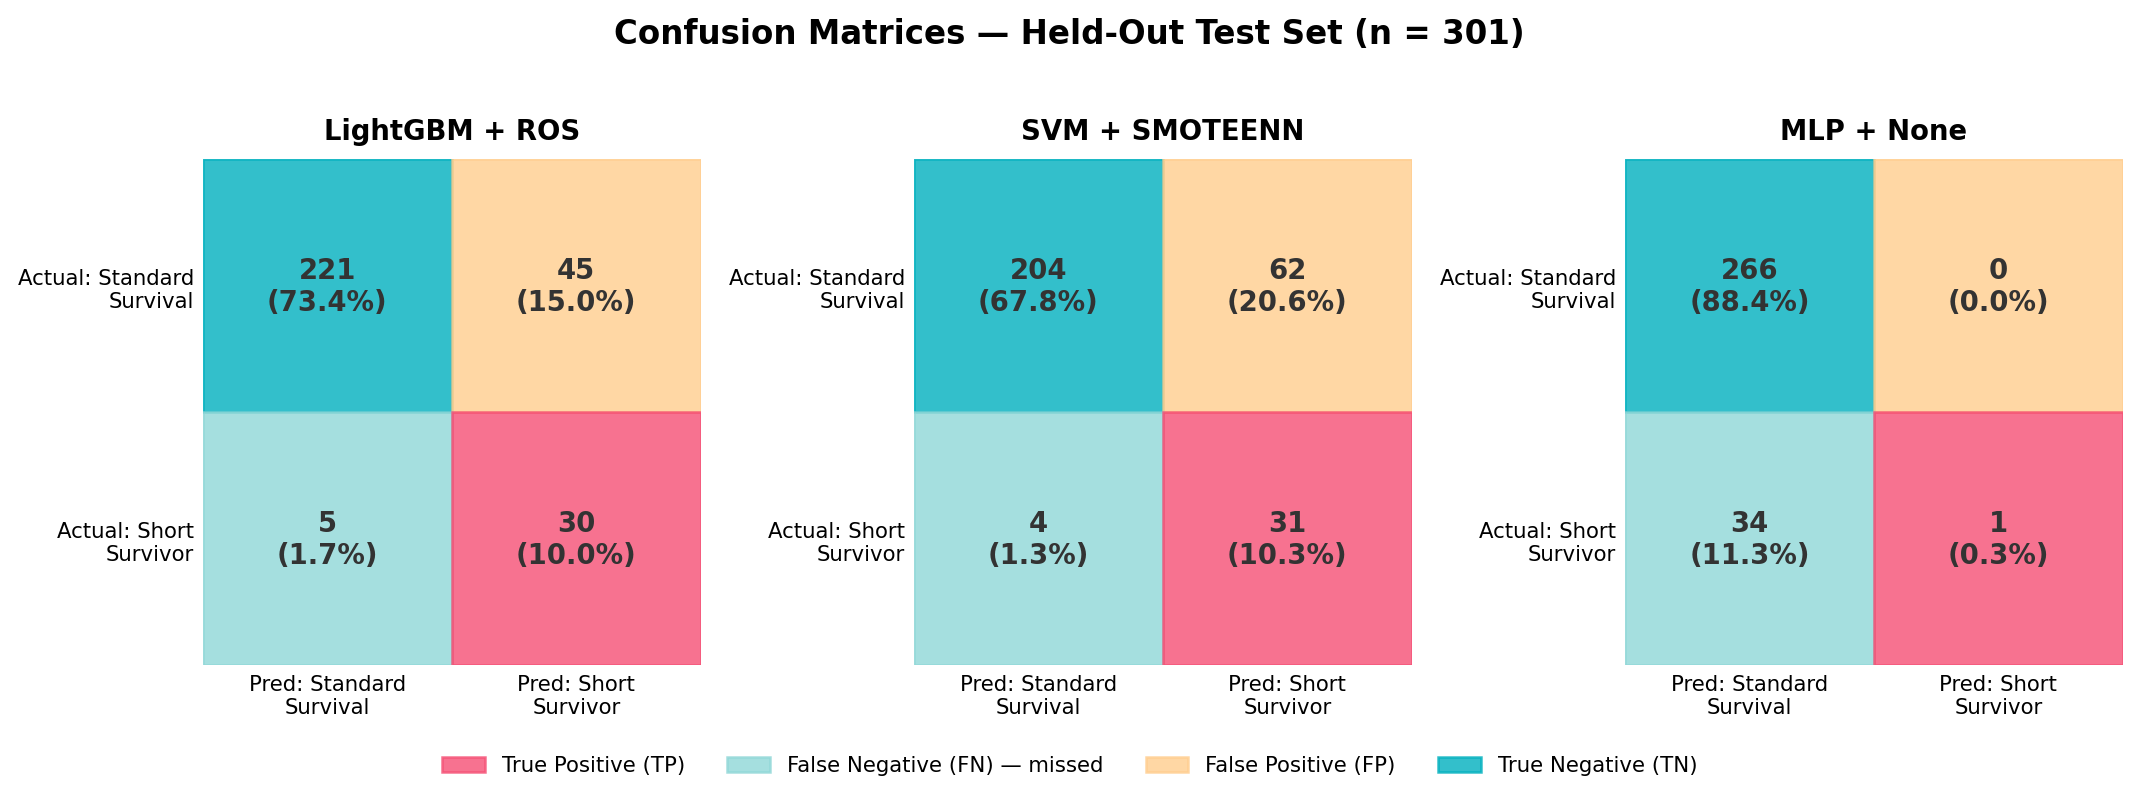
\includegraphics[width=0.97\linewidth]{figures/fig_confusion_matrices.png}
  \caption{Confusion matrices on the held-out test set for the three classifiers
    highlighted in the text. LightGBM+ROS and SVM+SMOTEENN correctly identify the
    majority of Short Survivors (TP), whereas MLP+None effectively classifies all
    patients as Standard Survival (FN$\,{=}\,$34).}
  \label{fig:cm}
\end{figure}
\clearpage

\subsection{Decision Threshold Analysis}
\label{subsec:threshold}

The AUC--sensitivity gap observed at the default 0.5 decision threshold
(Table~\ref{tab:test}) motivates a systematic investigation of alternative
operating points. Three thresholds were derived from out-of-fold (OOF) CV
predictions for each classifier---ensuring no information from the held-out test
set was used in their selection---and subsequently applied to the test set:
(i)~\textit{Youden's J}~\cite{youden1950} maximises sensitivity\,+\,specificity\,$-$\,1;
(ii)~\textit{sensitivity-optimised} targets the highest threshold achieving
$\geq 0.90$ sensitivity on OOF predictions; and
(iii)~\textit{F1-optimal} maximises minority-class F1 on OOF predictions.
Table~\ref{tab:threshold} reports results for the two most instructive classifiers.

\begin{table}[ht!]
  \caption{Test-set performance under three decision thresholds for MLP+None and
    LightGBM+ROS. Thresholds marked $\dagger$ were derived from out-of-fold CV
    predictions; the 0.50 row is the unmodified baseline from Table~\ref{tab:test}.
    The sensitivity-constrained strategy ($\geq 0.90$) returned degenerate thresholds
    ($\approx\!0$) for both classifiers, collapsing to predicting all patients as Short
    Survivors; it is excluded. TP\,/\,FN counts are out of 35 Short Survivors.}
  \label{tab:threshold}
  \resizebox{\linewidth}{!}{%
  \begin{tabular}{llcccccc}
    \toprule
    \textbf{Classifier} & \textbf{Threshold strategy} & \textbf{Threshold}
      & \textbf{Sensitivity} & \textbf{Specificity} & \textbf{Bal.\ Acc.}
      & \textbf{G-Mean} & \textbf{TP\,/\,FN} \\
    \midrule
    \multirow{3}{*}{MLP + None}
      & Default (0.50)       & 0.500 & 0.029 & 1.000 & 0.514 & 0.169 & 1\,/\,34 \\
      & Youden$^\dagger$     & 0.152 & 0.486 & 0.966 & 0.726 & 0.685 & 17\,/\,18 \\
      & F1-optimal$^\dagger$ & 0.239 & 0.371 & 0.981 & 0.676 & 0.604 & 13\,/\,22 \\
    \midrule
    \multirow{3}{*}{LightGBM + ROS}
      & Default (0.50)       & 0.500 & 0.857 & 0.831 & 0.844 & 0.844 & 30\,/\,5 \\
      & Youden$^\dagger$     & 0.404 & 0.857 & 0.778 & 0.818 & 0.817 & 30\,/\,5 \\
      & F1-optimal$^\dagger$ & 0.656 & 0.800 & 0.925 & 0.862 & 0.860 & 28\,/\,7 \\
    \bottomrule
  \end{tabular}%
  }
\end{table}

Lowering the MLP threshold from 0.500 to the Youden value (0.152) raises
sensitivity from 0.029 to 0.486---16 additional Short Survivors correctly
identified---while retaining high specificity (0.966). The F1-optimal threshold
(0.239) yields a more conservative recovery (sensitivity 0.371, specificity 0.981).
Even under optimal threshold selection, however, the MLP's best sensitivity (0.486)
remains well below that of LightGBM+ROS at the default boundary (0.857),
confirming that the AUC--sensitivity decoupling is structural rather than a
threshold artefact.

For LightGBM+ROS, the Youden threshold (0.404) detects the same number of Short
Survivors as the default (30 of 35), with a modest specificity trade-off (0.778
vs.\ 0.831). The F1-optimal threshold (0.656) shifts the balance toward specificity
(0.925), missing two additional patients (sensitivity 0.800), and yields the highest
G-Mean across all configurations in this table (0.860). Clinically, the choice
between these two operating points depends on whether minimising false negatives
or false positives is the priority.

The sensitivity-constrained analysis (targeting $\geq 0.90$ sensitivity) produced
degenerate thresholds ($\approx\!0$) for both classifiers on OOF predictions,
meaning no threshold achieves 90\% sensitivity with meaningful specificity under
the current feature set. This signals a dataset-level ceiling on Short Survivor
recall that neither resampling nor threshold selection can overcome without
additional discriminative features.

\subsection{BalancedBagging Replication and Statistical Validation}

To replicate the reference study, all seven classifiers were evaluated in
single-model and BalancedBagging configurations under the same cross-validation
protocol. Table~\ref{tab:bonferroni} reports mean balanced accuracy for each
condition along with the statistical comparison.

\begin{table}[ht!]
  \centering
  \caption{Cross-validation balanced accuracy under single-model and
    BalancedBagging configurations, with per-fold Wilcoxon signed-rank tests
    (Bonferroni-corrected for 7 comparisons).
    $^{***}p \leq 0.001$; $^{**}p \leq 0.01$; n.s.\ = not significant.}
  \label{tab:bonferroni}
  \resizebox{\linewidth}{!}{%
  \begin{tabular}{lcccc}
    \toprule
    \textbf{Classifier} & \textbf{Single-Model} & \textbf{BalancedBagging}
      & \textbf{$\Delta$} & \textbf{$p$ (Bonf.)} \\
    \midrule
    KNN           & 0.566 & 0.788 & $+$0.221 & $<0.001^{***}$ \\
    Naïve Bayes   & 0.797 & 0.809 & $+$0.012 & $>$0.999 n.s.  \\
    Decision Tree & 0.653 & 0.777 & $+$0.125 & $0.001^{**}$   \\
    Random Forest & 0.629 & 0.814 & $+$0.185 & $<0.001^{***}$ \\
    SVM           & 0.500 & 0.793 & $+$0.293 & $<0.001^{***}$ \\
    MLP           & 0.698 & 0.832 & $+$0.134 & $<0.001^{***}$ \\
    LightGBM      & 0.692 & 0.820 & $+$0.128 & $<0.001^{***}$ \\
    \bottomrule
  \end{tabular}%
  }
\end{table}

Six of the seven classifiers exhibit a statistically significant improvement in
balanced accuracy under BalancedBagging ($p \leq 0.01$ after Bonferroni
correction). The sole exception is Naïve Bayes ($p > 0.999$, n.s.): its generative
modelling of class-conditional densities makes it relatively insensitive to
training class proportions, and its single-model balanced accuracy (0.797) already
approaches its ensemble counterpart (0.809). The SVM shows the largest absolute
gain ($\Delta = +0.293$), crossing from a balanced accuracy of 0.500 to 0.793
once internal balancing is applied within each bootstrap sample. The MLP achieves
the highest ensemble balanced accuracy across all classifiers (0.832), consistent
with the reference study's findings. LightGBM also improves significantly under
BalancedBagging ($\Delta = +0.128$, $p < 0.001$), demonstrating that the ensemble
strategy generalises beyond the six classifiers considered in the original work.

\subsection{Comparison with the Reference Study}

Table~\ref{tab:comparison} summarises the methodological and performance
differences between the reference study and this work.

\begin{table}[ht!]
  \centering
  \caption{Direct comparison between Papaiz et al.~\cite{Papaiz2024} and this
    work. \textsuperscript{a}Best ensemble balanced accuracy reported under
    repeated CV. \textsuperscript{b}Not reported in the reference study.}
  \label{tab:comparison}
  \resizebox{\linewidth}{!}{%
  \begin{tabular}{lcc}
    \toprule
    \textbf{Aspect} & \textbf{Papaiz et al.~\cite{Papaiz2024}} & \textbf{This Work} \\
    \midrule
    Patients                    & 1,967              & 1,502              \\
    Classifiers evaluated       & 6                  & 7 (+LightGBM)      \\
    Imbalance strategies        & BalancedBagging    & 10 strategies + BB \\
    Hyperparameter optimisation & Grid search        & Bayesian (Optuna)  \\
    Best CV Bal.\ Acc.\ (MLP+BB)\textsuperscript{a} & $\approx$0.84 & 0.832 \\
    Held-out test evaluation    & No\textsuperscript{b} & Yes             \\
    Best test AUC               & ---\textsuperscript{b} & 0.923 (LightGBM+ROS) \\
    Best test Sensitivity       & ---\textsuperscript{b} & 0.857 (LightGBM+ROS) \\
    Explainability (SHAP)       & Yes (6 classifiers) & Yes (TreeSHAP + KernelSHAP) \\
    \bottomrule
  \end{tabular}%
  }
\end{table}

The CV balanced accuracy for MLP+BalancedBagging (0.832) comes close to the
reference figure ($\approx$0.84) on a smaller, more imbalanced cohort.
Three additions matter. Bayesian optimisation finds
hyperparameter configurations---particularly the MLP's high L2 penalty---that
grid search would rarely reach. LightGBM adds a gradient-boosted option the
original study did not test. And the held-out set reveals that MLP's
cross-validation lead does not hold under unseen data.

\subsection{Feature Importance via SHAP}

Figure~\ref{fig:shap} shows the TreeSHAP output for LightGBM+ROS on the held-out
test set, with features ranked by mean absolute SHAP value.

\begin{figure}[ht!]
  \centering
  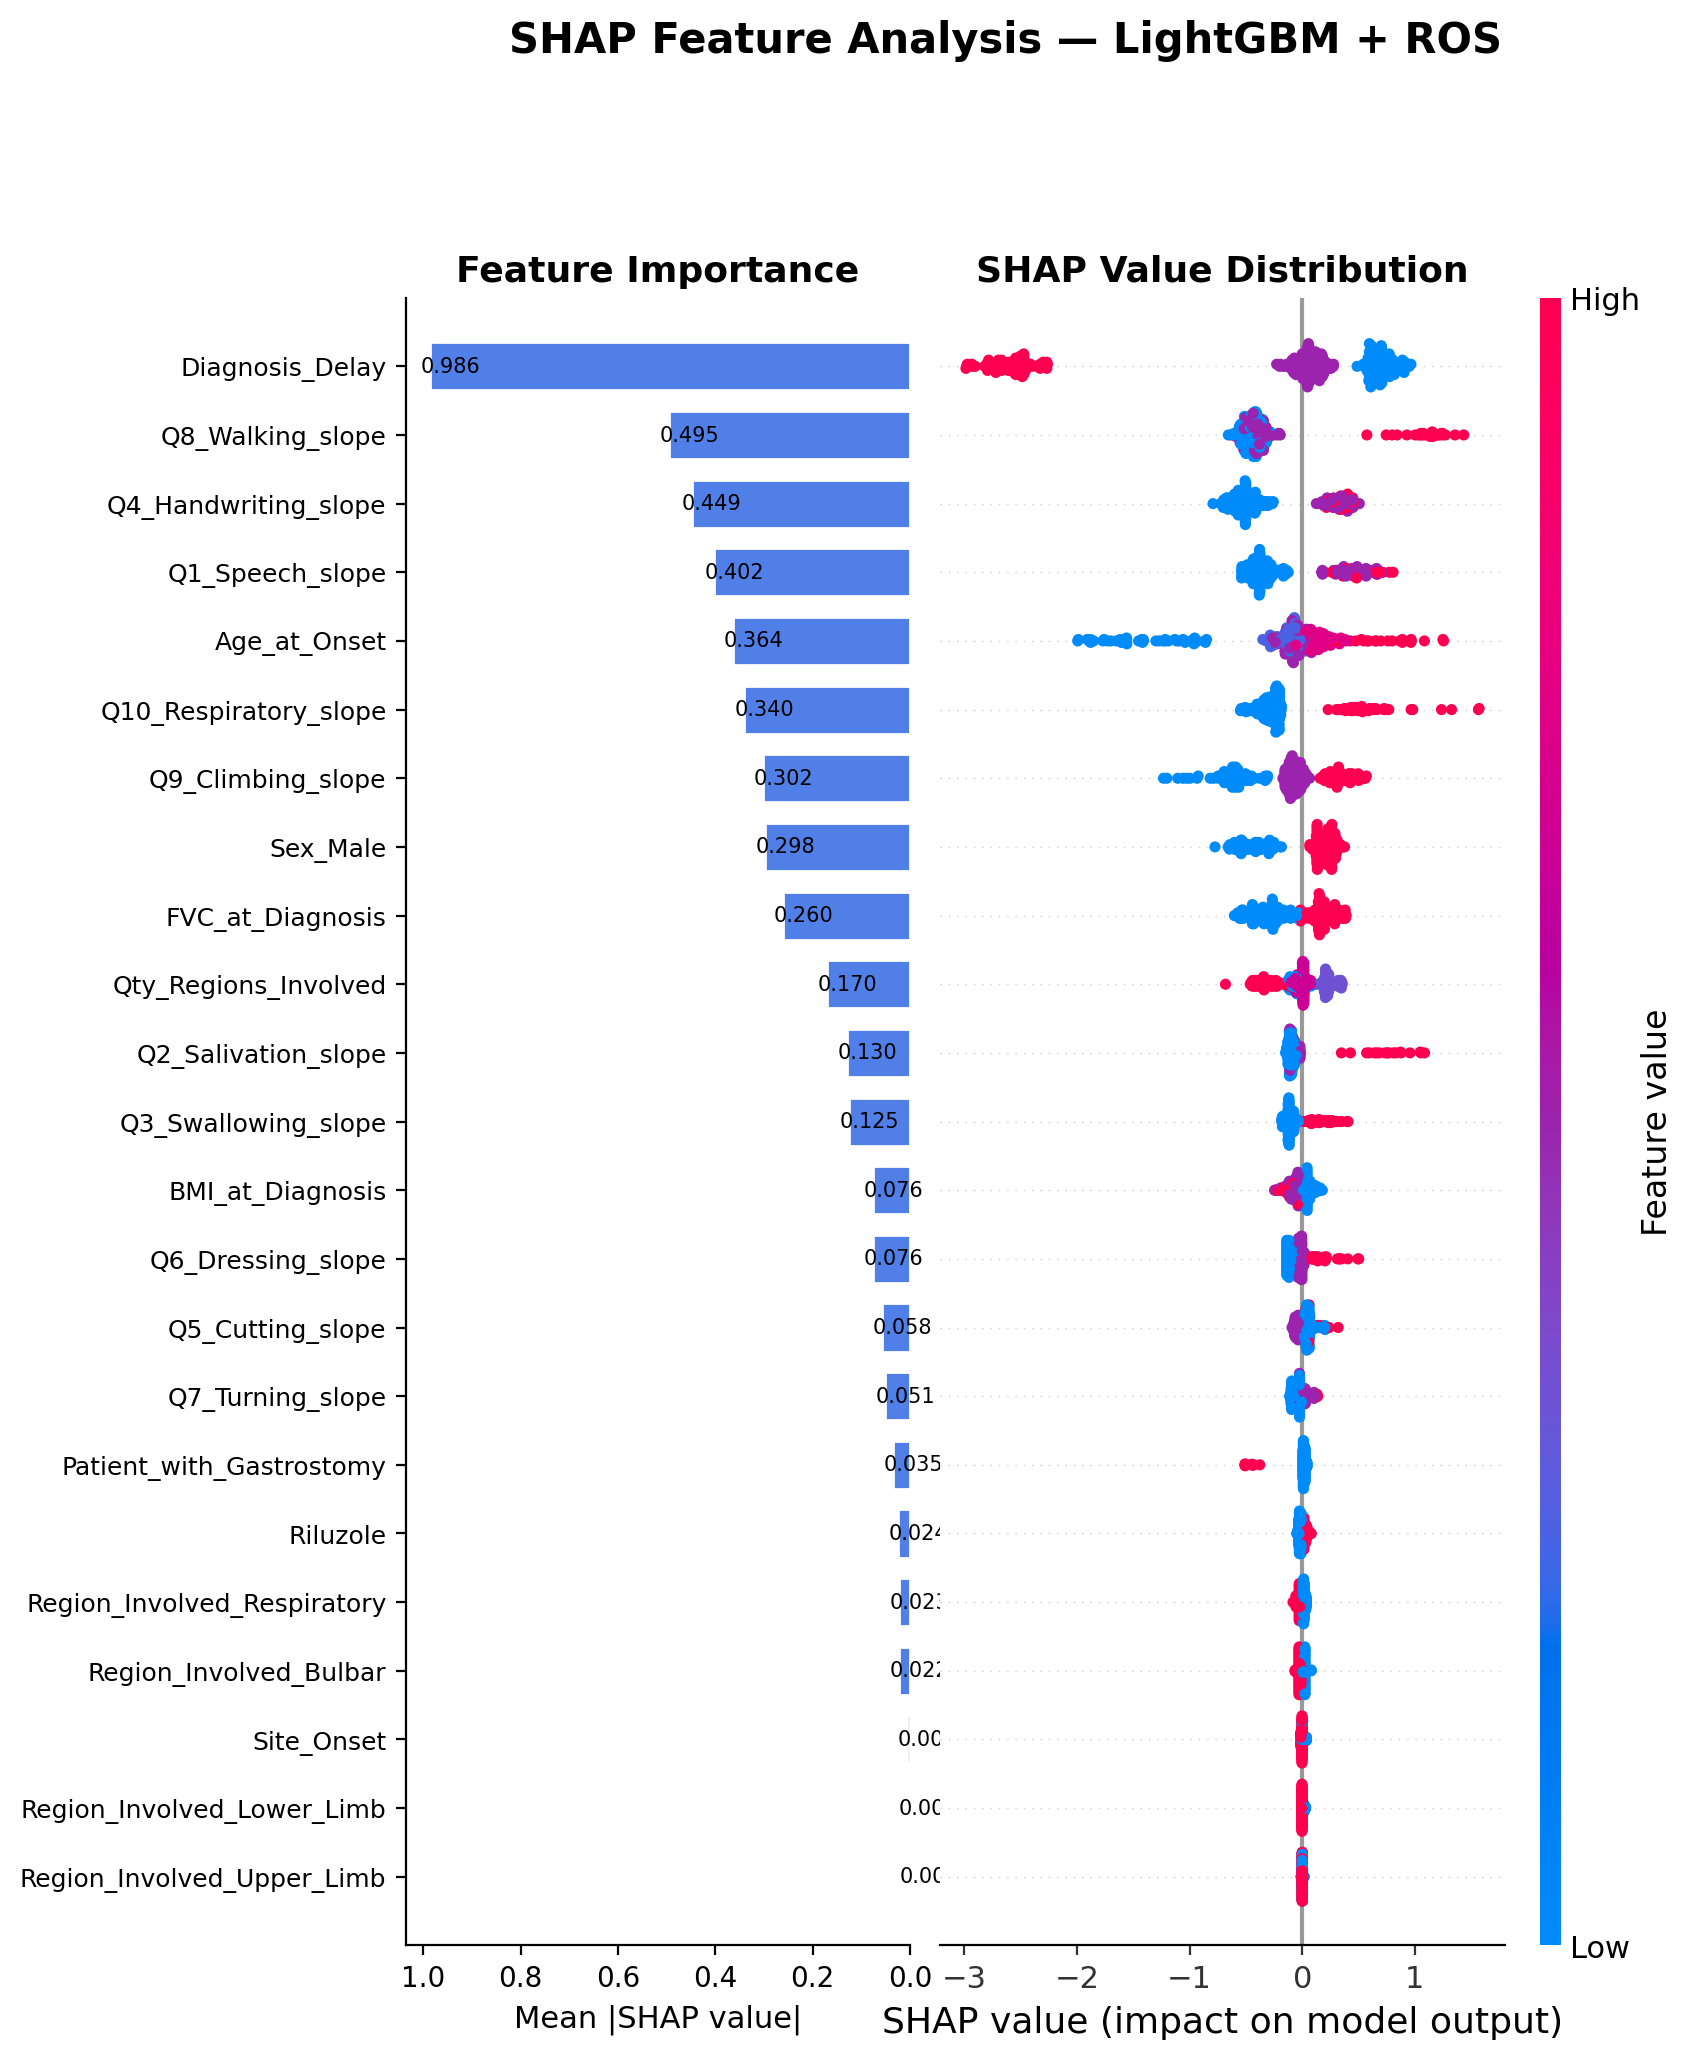
\includegraphics[width=0.95\linewidth]{figures/step7_lightgbm_fig3_combined.png}
  \caption{SHAP feature importance for LightGBM+ROS (held-out test set).
    \textit{Left:} global bar chart of mean $|\text{SHAP}|$ values.
    \textit{Right:} beeswarm plot showing per-instance SHAP contributions,
    coloured by feature value (red = high, blue = low).}
  \label{fig:shap}
\end{figure}

\texttt{Diagnosis\_Delay} is the dominant predictor (mean $|\text{SHAP}| = 0.986$),
more than double the next-ranked feature. Long delays associate with Standard
Survival; short delays signal rapid pre-diagnosis progression and Short Survivor
risk, consistent with clinical observations~\cite{Feldman2022}.

ALSFRS-R slopes fill ranks two through four and six: Q8 (walking), Q4
(handwriting), Q1 (speech), Q10 (respiratory). Age at onset is fifth
($|\text{SHAP}| = 0.364$); older patients tend to progress faster. FVC at
diagnosis ranks ninth ($|\text{SHAP}| = 0.260$), adding a respiratory
dimension. The ranking matches the reference study's SHAP output closely~\cite{Papaiz2024}.

The parallel KernelSHAP analysis of the MLP found the same top feature and a
broadly similar slope ranking, though with smaller absolute attributions (expected
given the more diffuse weight structure of neural networks).
Figure~\ref{fig:featbars} shows how \texttt{Diagnosis\_Delay} and Q8 separate
the two groups at the population level.

\clearpage
\begin{figure}[ht!]
  \centering
  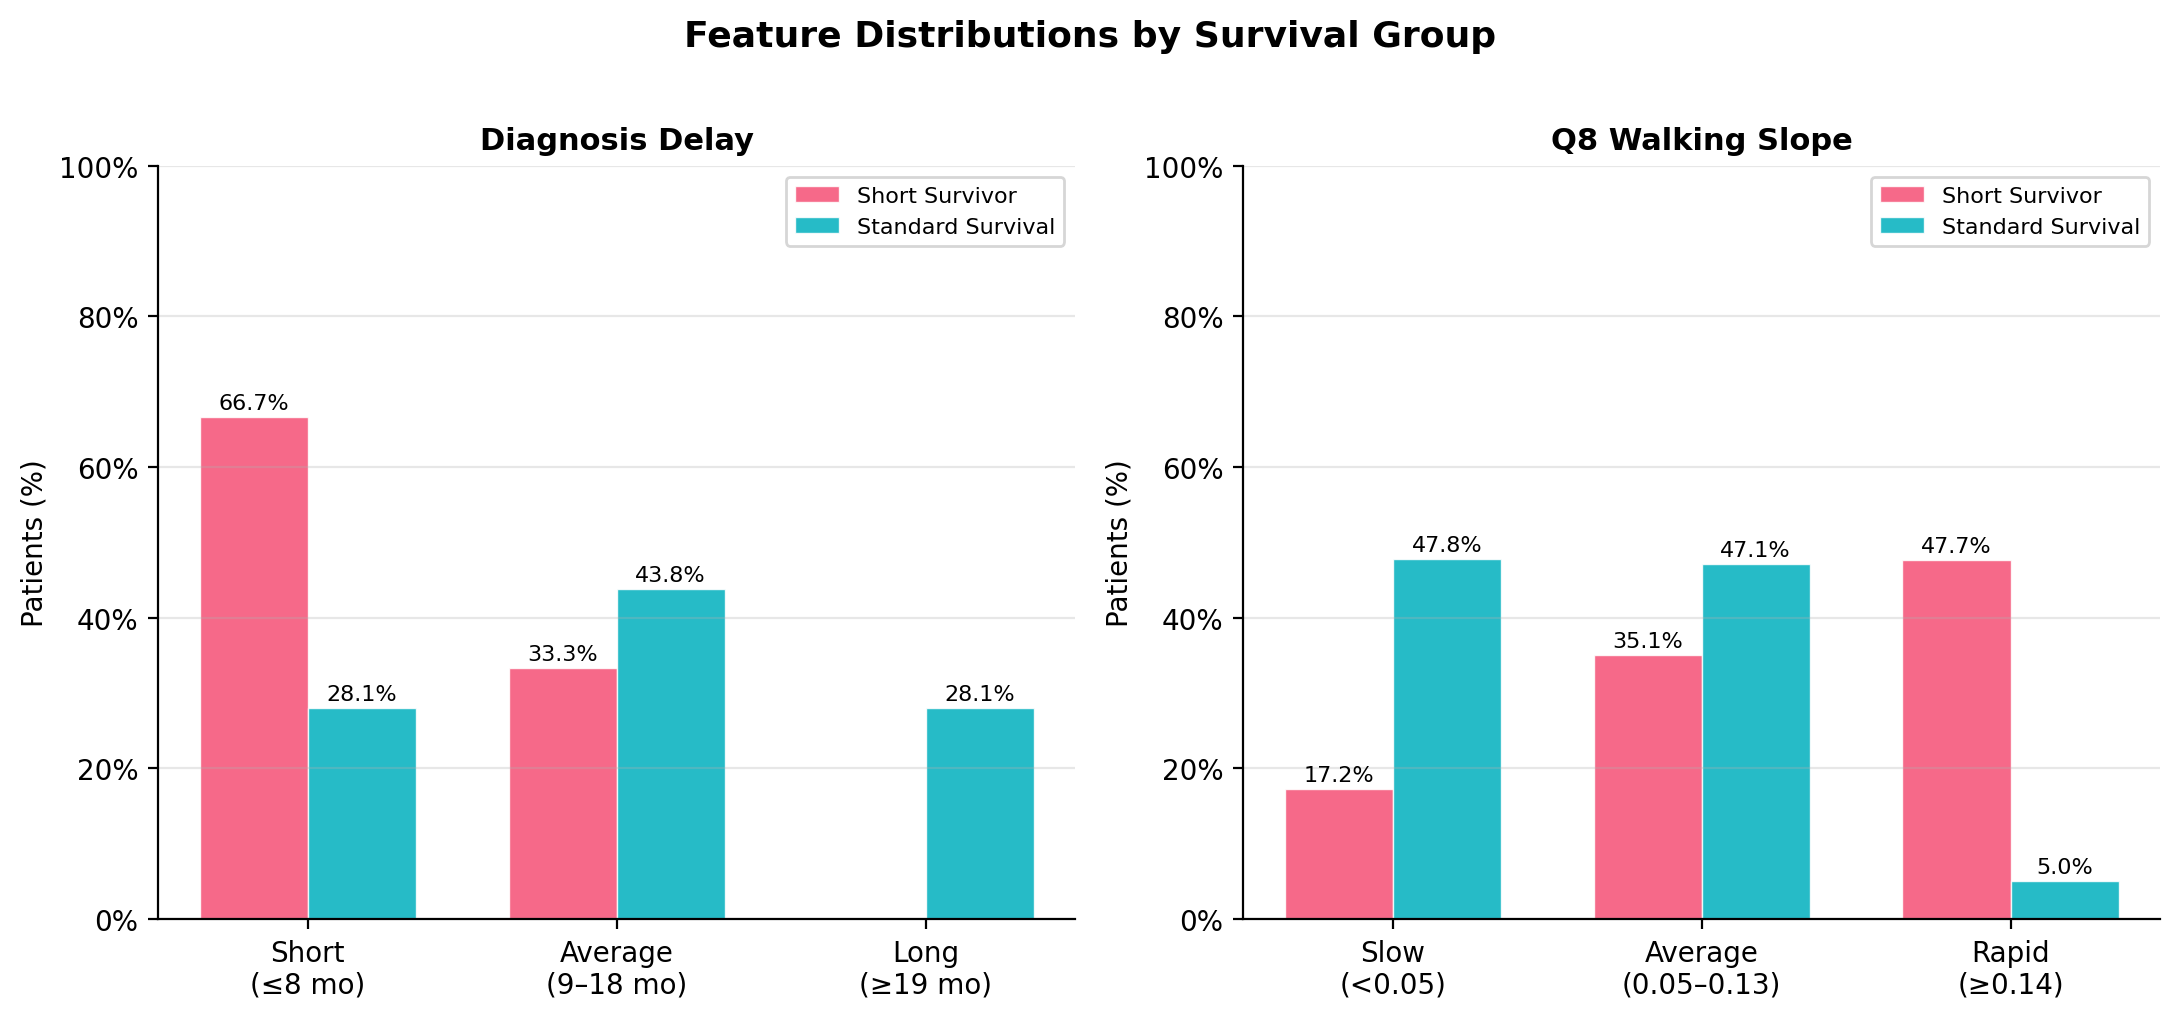
\includegraphics[width=0.97\linewidth]{figures/fig_feature_bars.png}
  \caption{Distribution of \texttt{Diagnosis\_Delay} (left) and
    \texttt{Q8\_Walking\_slope} (right) by survival group across the full
    dataset. Short Survivors are disproportionately concentrated in the
    short-delay and rapid-slope categories, consistent with their SHAP
    importance rankings.}
  \label{fig:featbars}
\end{figure}

% ==========================================================================
\section{Discussion}
\label{sec:discussion}
% ==========================================================================

\subsection{Replication Fidelity}

The central result of Papaiz et al.~\cite{Papaiz2024} holds: BalancedBagging
consistently improves balanced accuracy across classifiers, and the MLP reaches
0.832 versus the reference's $\approx$0.84. The gap is small. It reflects a
smaller cohort (1,502 versus 1,967 patients), a higher imbalance ratio (7.6
versus 6.9), and minor differences in the PRO-ACT extract we used. The
per-classifier pattern of gains mirrors the original paper across all seven
classifiers, including LightGBM, which was not in the reference study.

\subsection{Dataset Constraints and Potential Exclusion Bias}

Our PRO-ACT extract yielded 1,502 patients, 23.6\% fewer than the 1,967
in the reference study~\cite{Papaiz2024}. FVC missingness explains most of
this: 62.3\% of patients lacked a usable FVC record after applying the
survival and site-of-onset filters; without FVC, the 23-feature set defined by
the reference protocol cannot be fully instantiated.

This exclusion is unlikely to be random, and its directionality raises a
specific concern. FVC declines as disease progresses, and patients with rapid
early respiratory involvement---precisely those most likely to be Short
Survivors---are also the most likely to have attended fewer clinic visits, to
have had measurements recorded only in later stages, or to have been lost to
follow-up before a clean baseline FVC could be obtained. Excluding these patients
may therefore have shifted the cohort systematically towards less severe, more
slowly progressing cases, and may have underrepresented Short Survivors relative
to their true prevalence. If this systematic exclusion holds, the classification
task presented here is somewhat easier than it would be on a fully observed
population: the boundary between classes may be sharper and the minority class
less heterogeneous. Reported performance figures may consequently be optimistic,
and the actual sensitivity achievable in routine clinical deployment could be lower.

The reduced cohort size also directly degrades the precision of held-out
estimates. With only 35 Short Survivors in the test set, a change of two
predictions shifts sensitivity by 5.7 percentage points. Apparent differences
between models that look clinically meaningful should therefore be interpreted
cautiously: bootstrap confidence intervals around these point estimates would be
wide, and several pairwise comparisons may not reach statistical significance
under formal testing. These constraints do not invalidate the findings, but they
argue strongly against treating the reported metrics as precise absolute
benchmarks. Replication on a more complete PRO-ACT extract, or with principled
imputation strategies for missing FVC, is a clear priority for future work.

\subsection{The MLP Generalisation Problem}

The MLP's cross-validation AUC was 0.915 (first place). On the held-out test,
it identified one Short Survivor out of 35. AUC on the same test data: 0.918.
The model ranks patients' risk correctly on average; it assigns minority-class
scores that stay below 0.5. AUC measures ranking, not detection at a threshold.

A plausible interpretation: under severe imbalance, a model can assign slightly
higher probabilities to Short Survivors on average while those probabilities
never breach 0.5. Cross-validation detects the ranking signal. It does not
expose the threshold mismatch. The precision-recall curves in Figure~\ref{fig:pr} already provide a
threshold-independent view of the MLP's performance profile.
Section~\ref{subsec:threshold} demonstrates this directly: lowering the threshold
to the Youden optimum (0.152) raises the MLP's test sensitivity from 0.029 to
0.486, allowing 17 of 35 Short Survivors to be identified. Yet this remains well
below LightGBM+ROS at the default threshold (0.857), confirming that the
decoupling is structural and not merely a calibration artefact.

These results suggest that, in the presence of severe class imbalance, AUC alone
does not reliably reflect minority-class detection. Metrics that directly penalise
minority-class errors---sensitivity, balanced accuracy, G-Mean---should be part
of both the optimisation objective and the final evaluation; a held-out test,
even when internal, helps expose this gap.

\subsection{Advantages of LightGBM and Bayesian Optimisation}

LightGBM with Random Oversampling reached AUC 0.923, balanced accuracy 0.844,
and sensitivity 0.857 (30 of 35 Short Survivors correctly identified).
SVM with SMOTEENN reached sensitivity 0.886 (31 of 35) but at lower specificity
(0.767) and AUC (0.909); a usable alternative when missing a Short Survivor
is the dominant concern. Gradient boosting corrects residuals sequentially,
which helps it focus progressively on hard-to-classify minority instances.
Random Oversampling reinforces this by rebalancing the training set before fitting.

Bayesian optimisation with Optuna (TPE, 50 trials) allocated more search budget
to promising hyperparameter regions as information accumulated, something grid
search cannot do. This mattered most for LightGBM, whose search space is larger
than that of simpler classifiers.

TreeSHAP produces exact Shapley values for LightGBM in polynomial time.
KernelSHAP, used for the MLP, is approximate, needs 100 background samples
and 200 evaluation samples, and is susceptible to sampling variance. The
difference is not incidental: for clinical interpretability, exactness has value.

\subsection{Limitations}

The available PRO-ACT extract yields 1,502 patients, 23.6\% fewer than the
original study, primarily due to missing FVC records, which constrains statistical
power and may inflate variance in cross-validation estimates. The exclusion of
patients with missing FVC, height, or censored follow-up may further introduce
selection bias: missingness in clinical records is rarely random, and patients
too ill to complete assessments---and therefore more likely to be Short
Survivors---may be disproportionately absent, potentially shifting the retained
cohort towards milder disease trajectories. With an imbalance ratio of 7.6,
minority-class metrics are also sensitive to small changes in the confusion
matrix: a shift of two or three predictions can move sensitivity by several
percentage points. PRO-ACT participants were enrolled in controlled clinical
trials and may differ from community ALS patients in disease stage, comorbidity
profile, and duration of follow-up. Critically, the held-out test set is drawn
from the same PRO-ACT trial population as the training data; it provides an
unbiased estimate of in-distribution performance but does not replace external
validation on independent cohorts, which remains a necessary condition before
these models could inform clinical decisions. The AUC values reported here
(around 0.92) are strong for a 23-feature categorical model; while their
consistency across cross-validation and held-out evaluation argues against simple
overfitting, they may in part reflect structural properties specific to the
PRO-ACT trial population, and independent replication is needed before
generalisation can be assumed. ALSFRS-R decline slopes were extracted at the
assessment closest in time to each patient's diagnosis date; where no
pre-diagnosis visit existed, the nearest post-diagnosis assessment was used,
introducing a limited risk of temporal leakage for a subset of patients, a
limitation shared with the reference study. Statistical testing was limited to
the single-model versus BalancedBagging comparison; differences in performance
between individual classifiers were not formally tested and should be interpreted
descriptively rather than as statistically confirmed. The feature set, while
faithfully reproduced from the reference study, represents each patient at a
single time point through categorical and ordinal encodings; richer longitudinal
representations and biomarker data are not captured.

% ==========================================================================
\section{Conclusion}
\label{sec:conclusion}
% ==========================================================================

This work partially replicates and extends the ensemble-imbalance framework of Papaiz
et al.~\cite{Papaiz2024} with Bayesian hyperparameter optimisation
and LightGBM. The replication holds: across six of seven classifiers,
BalancedBagging produces statistically significant gains in balanced accuracy
($p \leq 0.01$, Bonferroni-corrected), and the MLP reaches an ensemble balanced
accuracy of 0.832, close to the reference's $\approx$0.84.

The held-out evaluation, drawn from the same PRO-ACT trial population, adds three
observations. First, the MLP's leading cross-validation AUC (0.915) does not
translate to minority-class detection at the default threshold: sensitivity falls
to 0.029, which reflects an AUC--sensitivity decoupling rather than an absence of
discriminative signal. Second, LightGBM with Random Oversampling achieves the best
overall balance across metrics (AUC 0.923, sensitivity 0.857, balanced accuracy
0.844); SVM with SMOTEENN reaches higher raw sensitivity (0.886) at lower
specificity (0.767) and is the better choice when missing a Short Survivor
is the dominant concern. Third, SHAP analysis of both models consistently identifies
diagnostic delay and ALSFRS-R decline slopes as the dominant predictors.

These results carry three methodological implications. AUC alone does not
reliably surface minority-class failures under severe imbalance. Threshold
selection belongs inside the evaluation, not left at 0.5 by default. And a
held-out test, even when internal, exposes gaps that cross-validation rankings
conceal. External validation on cohorts independent of
PRO-ACT remains necessary before these findings can be applied in practice.
Future work should address threshold calibration and cost-sensitive learning,
richer longitudinal feature representations, and validation on independent cohorts.

\textbf{Technical notes:}
All experiments were implemented in Python~3.12 using scikit-learn~1.8~\cite{pedregosa2011scikit}, LightGBM~4.6~\cite{ke2017lightgbm}, Optuna~4.8~\cite{akiba2019optuna}, imbalanced-learn~\cite{lemaitre2017}, and SHAP~\cite{lundberg2017shap}. All computations were performed on a standard CPU environment; no GPU acceleration was required.


\section*{Code Availability}
The analysis code, pre-processed outputs, and figure generation scripts are
publicly available at \url{https://github.com/NotAnnieMore/ThesisReplication}
under the MIT Licence.
Raw PRO-ACT data are not included due to the Data Use Agreement governing
access to the PRO-ACT database; they can be requested at
\url{https://ncri1.partners.org/ProACT}.

\section*{Acknowledgment}
This work is funded by national funds through the FCT - Foundation for Science and Technology, I.P., within the scope of the project CISUC - UID/CEC/00326/2020 and by European Social Fund, through the Regional Operational Program Centro 2020 and by the Portuguese Research Agency FCT, through D4 - Deep Drug Discovery and Deployment (CENTRO-01-0145-FEDER-029266). Maryam Abbasi thanks the National funding by FCT - Foundation for Science and Technology, P.I., through the institutional scientific employment program-contract (CEECINST/00077/2021).\\

\textbf{Declaration of generative AI and AI-assisted technologies in the writing process}

During the preparation of this work the author(s) used ChatGPT in order to gain insights and assistance in structuring and organizing the content, enhancing clarity, and refining specific sections. After using this tool/service, the author(s) reviewed and edited the content as needed and take(s) full responsibility for the content of the publication.
 
\bibliographystyle{elsarticle-num} 
\bibliography{bibfile}

\end{document}